\graphicspath{{chapters/3_diseño/figures/}}

% parte central
\chapter{Voxel cone tracing}\label{chap:design}

En este capítulo se detalla el diseño de \textit{voxel cone tracing} \cite{voxel-cone-tracing}, un algoritmo de iluminación global en tiempo real, que utiliza conceptos presentes en el trazado de rayos \ref{sec:ray-tracing} y \textit{photon mapping} \ref{sec:photon-mapping}.
Reduce los costos asociados a estos algoritmos clásicos de trazado de rayos utilizando vóxeles \ref{sec:voxels}, \textit{octrees} dispersos \ref{sec:octree} y conos \ref{sec:cone-marching}.

% TODO: Debería definir el tema de los conos en el capítulo 2.
% Puedo sacar información en la tésis de Crassin.
% Papers que voy encontrando del tema:
% - Ray tracing with cones - Amanatides '84
% - El resto no están disponibles
% Parece que el tema de anti-aliasing es muy importante.
% A nosotros no nos importa esa aplicación de los conos, pero podemos mencionarla sin duda

Para lograr el renderizado en tiempo real, \textit{voxel cone tracing} realiza aproximaciones.
Una de ellas es el uso del ducto de raster visto en la sección \ref{sec:graphics-pipeline}.
Los cálculos de luz se realizan en el \textit{fragment shader} del ducto de raster.
Esto difiere del trazado de rayos clásico, que renderiza toda la escena puramente mediante intersecciones entre rayos y geometría.

También se utiliza el renderizado diferido, visto en la sección \ref{sec:deferred-rendering}, para reducir la cantidad de vértices sobre los que se realizan cálculos.

La principal aproximación que realiza el algoritmo es la de 



El trazado de conos se usa para agregar efectos de iluminación global a una escena rasterizada utilizando mallas poligonales para sus superficies.

Para reducir la cantidad de cálculos a realizar, se utiliza una aproximación de la escena, en la forma de vóxeles almacenados en el \textit{octree}.
Al calcular la radiancia de la escena que incide en un punto, se utiliza un nivel de detalle menor de cada parte de la escena, cuanto más alejada se encuentre del punto.
Debido a esto, en lugar de trazar rayos, que mantienen el mismo tamaño a medida que se aleja de su punto de origen, se trazan conos, cuyo diámetro crece a medida que se aleja de su origen.
% TODO: Imagennn. Seguramente acá podamos usar el debug cone
Mientras más lejos el punto muestreado del origen del cono, más grande el diámetro del mismo.
Este tamaño se usa para determinar qué nivel de detalle será utilizado para esta región de la escena.
Este nivel de detalle se almacena en un \textit{octree} disperso.

Para generar esta estructura, se voxeliza la escena y se usan los vóxeles como base para el \textit{octree}.
Luego, se promedian los valores de los vóxeles en el último nivel del \textit{octree} a los niveles superiores, de tal manera que cada nodo aproxime la región del espacio que le corresponde.

El algoritmo se puede dividir en 3 grandes etapas:

\begin{enumerate}
    \item Voxelización de la escena
    \item Construcción del \textit{octree} disperso
    \item Trazado de conos
\end{enumerate}

En el resto del capítulo se explicará con mayor grado de detalle cada una de estas etapas.

\section{Voxelización}

La escena se divide en una grilla de vóxels.
La cantidad de vóxels es configurable, siendo usualmente $512$ o $1024$ por dimensión.

Para voxelizar la escena, se realiza el procedimiento detallado en ``OpenGL Insights, capítulo 22'' \cite{opengl-insights}, un aporte que escribió Crassin luego de haber publicado el artículo de \textit{voxel cone tracing}, aprovechando mejoras en las herramientas disponibles en el momento.
Ese mismo proceso será explicado a continuación, para más información, consultar la referencia.

Usando la rendering pipeline de OpenGL, se voxelizan todos los triángulos de la geometría de la escena.
Esto genera una lista de \textbf{fragmentos de vóxel}, con atributos como posición y color.
Cada uno de estos fragmentos será usado para construir el SVO y terminará siendo un vóxel en la estructura.

La voxelización de un triángulo $B$ a un vóxel $V$ puede hacerse si:

\begin{enumerate}
    \item El plano de $B$ interseca $V$.
    \item La proyección 2D del triángulo $B$ por la dimensión dominante de su normal (la que provee la mayor área proyectada) interseca la proyección 2D de $V$.
\end{enumerate}

Basado en esta observación, se sigue la serie de pasos que se muestra en la figura \ref{fig:voxelization_pipeline}.

\begin{figure}[h!]
    \centering
    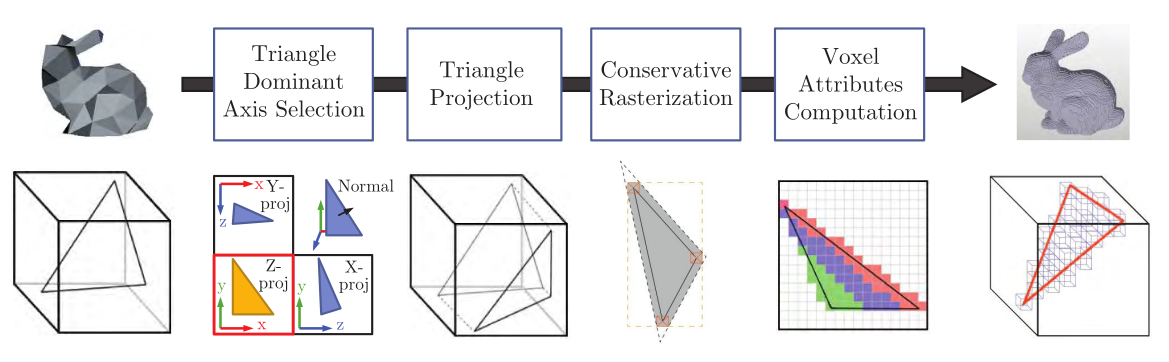
\includegraphics[width=\textwidth]{voxelization_pipeline.png}
    \caption{Ducto de voxelización. Fuente: \cite{opengl-insights}}
    \label{fig:voxelization_pipeline}
\end{figure}

Primero, cada triángulo de la geometría se proyecta ortográficamente en la dimensión dominante de su normal.
La dimensión dominante se elige dinámicamente por triángulo en el \textit{geometry shader}, donde la información de los tres vértices de cada triángulo está disponible.

Cada triángulo proyectado se rasteriza para conseguir fragmentos correspondientes a la resolución 3D de la grilla de vóxels.
Se fija el tamaño del \textit{viewport} a coincidir con la cantidad de vóxeles, por ejemplo un \textit{viewport} de tamaño $512\times512$ para una grilla de $512^3$ vóxeles.
% Mientras se hace esto, se mantienen las operaciones del framebuffer desactivadas, como el depth testing. % TODO: Habría que explicar por qué, no entendí del capítulo de OpenGL Insights

Durante la rasterización, cada triángulo genera un conjunto de fragmentos 2D.
Estos fragmentos pueden intersecar con a lo sumo 3 vóxeles de la grilla. % TODO: Por qué?
A su vez, debido a la elección de la dimensión dominante de la normal para la proyección, solo pueden intersecar con 3 vóxels en la profundidad también. % TODO: Por qué?
Entonces, por cada fragmento 2D, los vóxeles que intersecaron con el triángulo se calculan en el \textit{fragment shader}, basándose en la posición, la profundidad y las derivadas en espacio de pantalla. % TODO: Hacemos lo de las derivadas?

Esta información se usa para generar una lista de \textbf{fragmentos de vóxel}.
Estos son una generalización en 3D de los fragmentos 2D y corresponden a un vóxel que intersecta con un triángulo.
Cada fragmento de vóxel tiene una coordenada que lo identifica dentro de la grilla 3D de vóxels, así como color y posición.

\subsection{Rasterización conservativa}

El método descrito anteriormente a veces no crea fragmentos para elementos muy finos, como un asta de bandera.
Esto pasa porque solo se prueba el centro del píxel contra los triángulos para generar fragmentos. % TODO: Revisar en el código
Se necesita una manera de generar fragmentos para cada píxel tocado por un triángulo, no necesariamente en el centro.
Un algoritmo así se detalla en \cite{conservative-rasterization}.

La idea es generar, por cada triángulo, un polígono acotante ligeramente más grande, para asegurarse que cualquier triángulo proyectado que toca un triángulo (en cualquier punto) también toca su centro. % TODO: Esto es triángulo que toca un triángulo o que toca un vóxel/píxel?
Esto se hace alargando las aristas del triángulo hacia afuera.
Hay fragmentos que resultan de sobreestimar la cobertura de este triángulo, los cuales se descartan.
Este proceso se muestra en la figura \ref{fig:conservative_rasterization}.

% TODO: Cambiar por una foto nuestra?
\begin{figure}[h!]
    \centering
    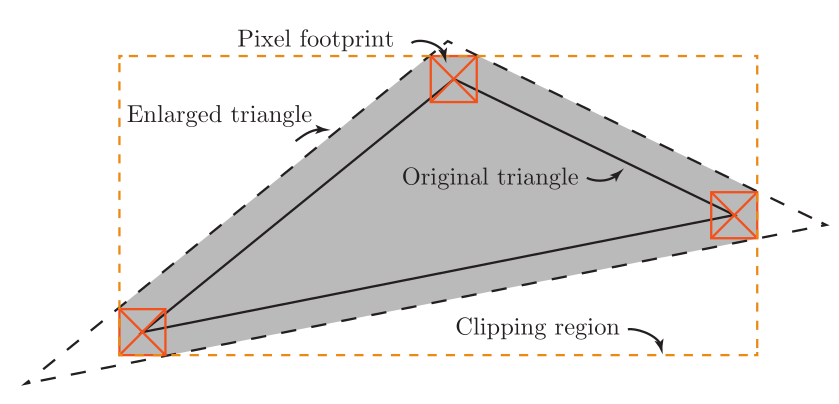
\includegraphics[width=\textwidth]{conservative_rasterization.png}
    \caption{Rasterización conservativa. Fuente: \cite{opengl-insights}}
    \label{fig:conservative_rasterization}
\end{figure}

\section{Sparse Voxel Octree}

Para almacenar los fragmentos de vóxeles generados, se usa un \textit{octree} disperso.
Esta estructura subdivide la escena en $8$ y cada hijo en $8$ y así sucesivamente.
Al ser disperso, puede ser que ciertos hijos no se subdividan si no hay más geometría dentro de la región de la escena que representan.

Cada elemento del árbol es un nodo.
Un nodo del árbol representa una sección de la escena.
Cada nivel tiene una cierta cantidad de nodos.
Si el árbol fuera denso, cada nivel $n$ tendría $8^n$ nodos.
El nivel $0$ tendría $1$, el nivel $1$ tendría $8$, el $2$ tendría $64$ y así sucesivamente.
En este caso, al ser un árbol disperso, no se crean nodos para regiones de la escena que no contienen geometría.
El último nivel del árbol es el que llega a la resolución deseada de $512$ o $1024$ vóxeles.
Valores más altos de resolución crean más niveles del \textit{octree} y se asemeja cada vez más la aproximación a la geometría real.

Dado que la estructura tiene como máximo $512$ o $1024$ vóxeles de resolución, sin importar la geometría de la escena, los cálculos sobre ella son independientes de la complejidad de la geometría.

\subsection{Nodos y bricks}\label{sec:nodes_and_bricks}

El SVO no solo está compuesto por los nodos del árbol.
A su vez, cada nodo tiene asociado un \textit{brick}, una estructura que también representa una región del espacio, pero que almacena valores distintos.
Cada nodo del árbol almacena únicamente un puntero a sus, como máximo $8$, hijos.
Los bricks almacenan los valores necesarios que representan esa región del espacio, por ejemplo el color.

Cada brick está dividido en 27, $3\times3\times3$, vóxeles.
Son estos vóxeles los que almacenan los valores de la escena.
En la figura \ref{fig:node_and_brick} se puede observar un nodo con su brick asociado de la manera en la que se disponen en el espacio.
Los bricks ocupan más espacio que sus nodos.
Esto es para que los bricks puedan obtener valores de sus vecinos, para garantizar que la interpolación dentro de un solo brick toma en cuenta a los vecinos.
Esto resulta en una frontera compartida entre vecinos, como se puede ver en la figura \ref{fig:brick_border_overlap}.
Esta frontera debe almacenar lo mismo para que la interpolación a la hora de generar la imagen final funcione.
Esto se logra mediante un programa llamado \textit{border\_transfer}, que se explicará en la sección \ref{sec:border_transfer}.

% TODO: Está buena la idea de marcar con italics la primera vez pero después no más. Hacerlo en todos lados.

\begin{figure}[h!]
    \centering
    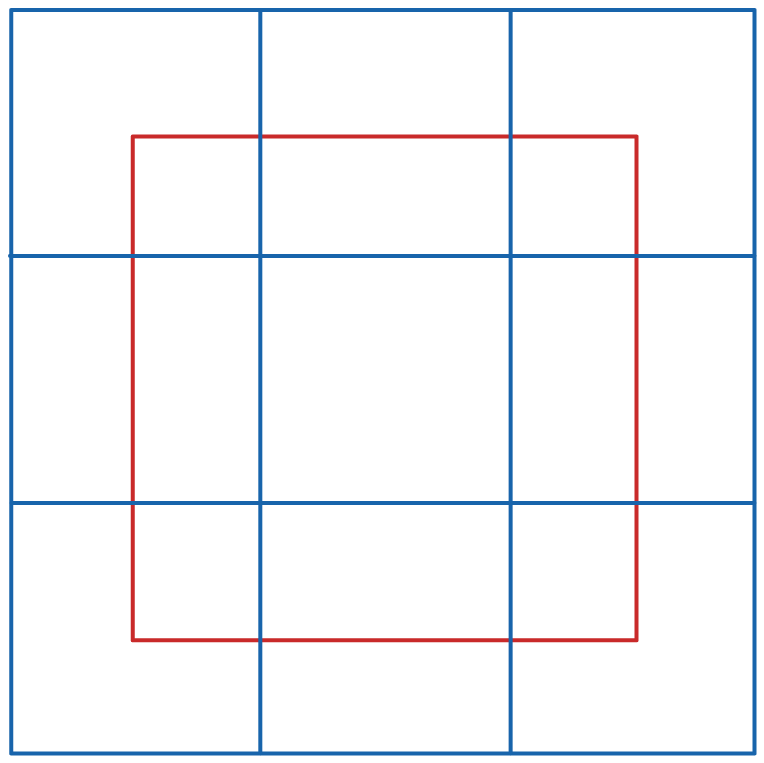
\includegraphics[width=.3\textwidth]{node-and-brick.png}
    \caption{Nodo con su brick asociado (en 2D)}
    \label{fig:node_and_brick}
\end{figure}

\begin{figure}[h!]
    \centering
    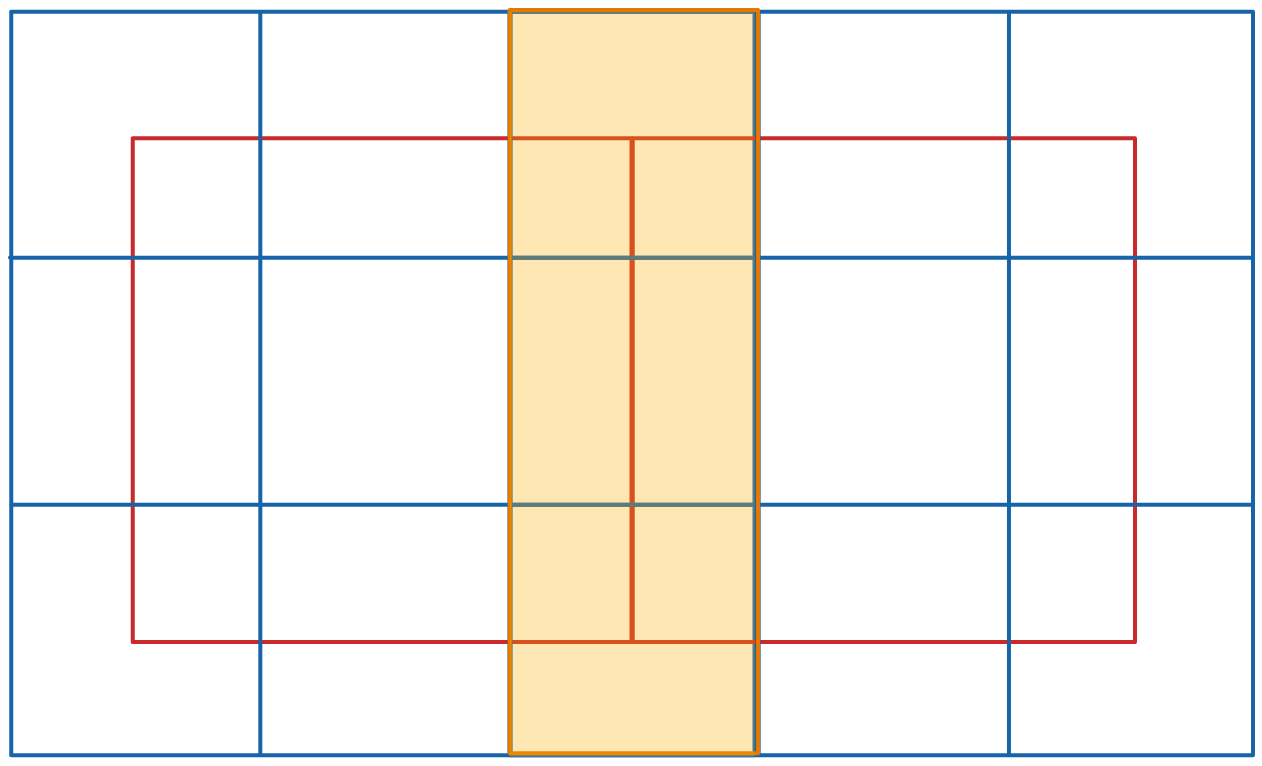
\includegraphics[width=.5\textwidth]{brick-border-overlap.png}
    \caption{Solapamiento entre vóxels de bricks de nodos vecinos}
    \label{fig:brick_border_overlap}
\end{figure}

\subsection{Construcción}\label{design:svo_construction}

Para generar esta estructura se usan los fragmentos de vóxeles.
Se empieza con un árbol con un solo nivel, con un solo nodo que ocupa toda la escena.
Se ejecuta el algoritmo a continuación sobre este nivel para generar el siguiente, y luego se continúa aplicándolo en cada nivel del árbol hasta completarlo.

Dado un nivel $i$ del árbol, dos programas principales son ejecutados en secuencia para generar el nivel $i + 1$: \textit{flag\_nodes} y \textit{allocate\_nodes}.

Se corre un hilo de \textit{flag\_nodes} por cada fragmento de la lista de fragmentos.
Dado un fragmento, se recorre el árbol construido hasta el momento, hasta que se llega a una sección del nodo no subdividida.
Esta sección del nodo se marca para ser subdividida.

Luego, se ejecuta \textit{allocate\_nodes}, que busca en el nivel $i$ marcas para subdividir.
Al encontrar una sección de un nodo marcada, crea un nuevo nodo en la estructura y cambia la marca por un puntero a ese nuevo nodo.

Siempre y cuando haya un fragmento en la región de la escena representada por un nodo, este será subdividido nivel tras nivel.

Una vez alcanzado el último nivel, se escriben los atributos de los fragmentos en los bricks de las hojas del árbol, promediando cuando más de uno cae en la misma hoja.
Esto último pasa más mientras más triángulos tiene la escena original y menos resolución tiene la grilla de vóxels.
Las hojas no tienen hijos.

En \ref{sec:nodes_and_bricks}, se vió como los bricks ocupan una región más amplia del espacio.
% TODO: Habría que explicar que los vóxeles son un octavo de nodo del último nivel. Para que esto tenga sentido.
Para consolidar esto con el tamaño de los fragmentos, estos se almacenan únicamente en las esquinas de los bricks.
Se almacenan en la esquina más cercana a la posición del fragmento.
Luego, se aplica un programa \textit{spread\_leaves}, para esparcir estos valores a lo largo de todo el brick.
Esto funciona de la siguiente manera, la cual se muestra en 2D en la figura \ref{fig:spread-leaves}:
\begin{itemize}
    \item El vóxel central almacena el promedio de todas las 8 esquinas
    \item El vóxel del medio de cada cara almacena el promedio de las 4 esquinas de su cara
    \item El vóxel del medio de cada arista almacena el promedio de las 2 esquinas de esa arista
\end{itemize}
De esta manera, se esparcen los valores de las esquinas a todo el brick.
Este es el algoritmo que expande los vóxeles generados poder llenar los bricks $3\times3\times3$.

\begin{figure}
    \begin{subfigure}{.5\textwidth}
        \centering
        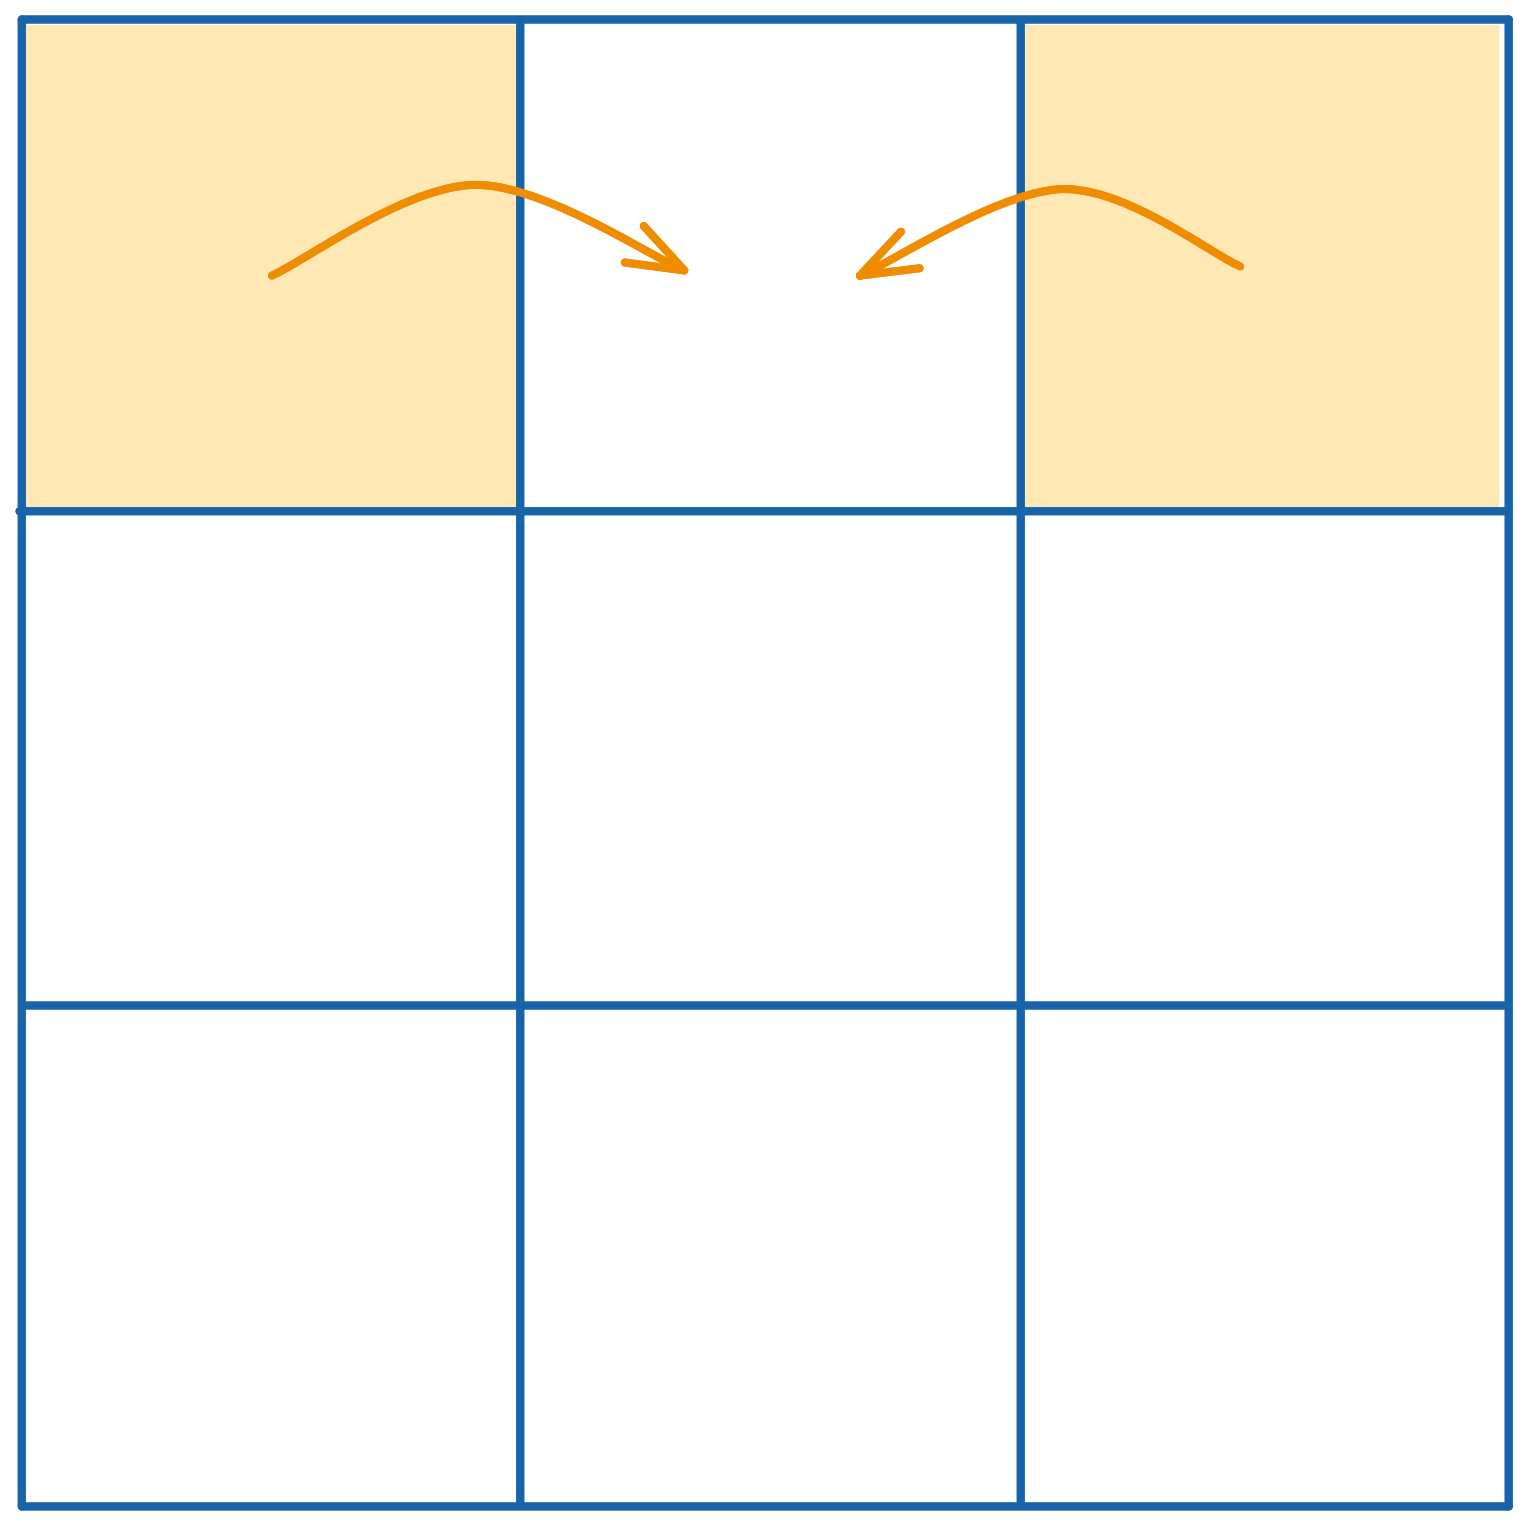
\includegraphics[width=.75\textwidth]{spread-leaves-edge.png}
        \caption{En una arista}
    \end{subfigure}
    \begin{subfigure}{.5\textwidth}
        \centering
        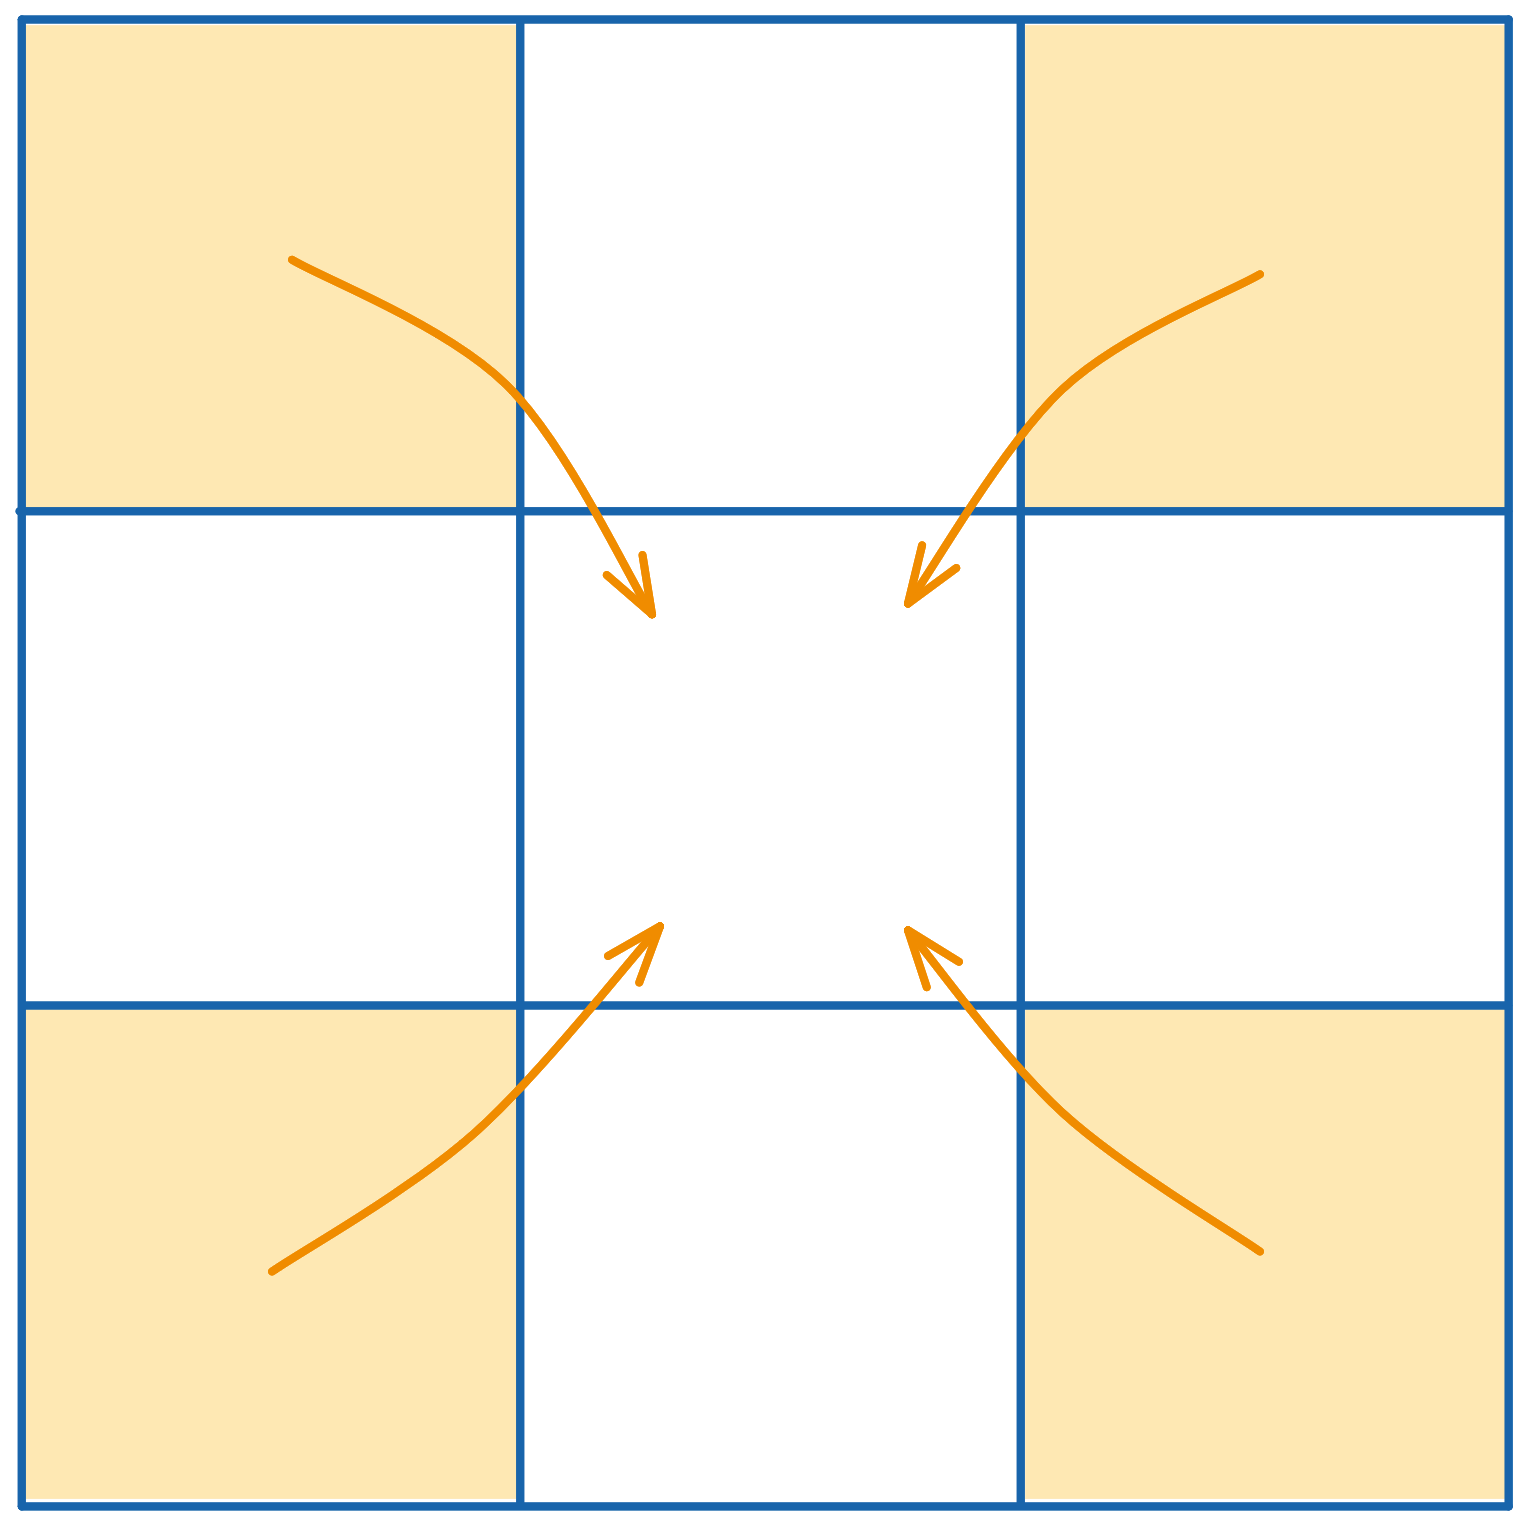
\includegraphics[width=.75\textwidth]{spread-leaves-center.png}
        \caption{En el centro}
    \end{subfigure}
    \caption{Funcionamiento de \textit{spread\_leaves} en 2D. Las flechas indican aporte al promedio}
    \label{fig:spread-leaves}
\end{figure}

% Explicando el writeLeaf, spread y borderTransfer

Como se mencionó anteriormente, las fronteras entre bricks son compartidas, corresponden al mismo espacio en la escena.
Por lo tanto, los valores almacenados en esos vóxels deben ser los mismos.
Para lograr esto, una vez que los valores son almacenados en cada brick, se transfieren los valores de la frontera al brick vecino, asegurandose que sea coherente el nivel.
En el caso del color y las normales, se guarda en las fronteras de cada brick, el promedio de estos valores.

% TODO: Qué es mejor usar? sec:algo, design:algo, sec:design:algo?
\subsection{Border transfer}\label{sec:border_transfer}

Recordar que los bricks comparten una frontera con sus vecinos.
Luego de \textit{spread\_leaves}, esta frontera tiene cosas distintas en cada brick vecino.
Es necesario que tengan el mismo valor para cada brick, para garantizar una suave interpolación a la hora de generar la imagen final.
De esto se encarga \textit{border\_transfer}.
Este programa promedia los valores en la frontera de cada brick con la de sus vecinos, en X, Y y Z.
De esta manera, aún cuando un vóxel puede estar en varios bricks, en $8$ como máximo, su valor va a ser siempre el mismo en cada uno de ellos.

% TODO: Creo que lo mejor sería renombrar los voxel fragments a simplemente voxels.

\subsection{Nodos frontera}

Al usar un octree disperso, no existen nodos donde no hay geometría.
Esto permite ahorrar memoria, pero tiene un problema.
A la hora de interpolar para generar la imagen final, esta interpolación de efectos logrados por el algoritmo, por ejemplo sombras y reflejos, solo llega hasta el final de los nodos existentes, luego se corta abruptamente.
Para que la interpolación continué y logre difuminar estos efectos, es preciso una capa de nodos extra, nodos frontera, entre la geometría y el espacio vacío.
Estos nodos se añaden en cada nivel del árbol a la hora de construírlo.
Sus bricks no contienen valores, existen solo para interpolar los valores con 0 y difuminar los bordes de la geometría.

% El algoritmo de cone tracing se ejecuta para cada punto visible de la escena y calcula un color.
% En el caso de oclusión ambiental, este color es un gris que representa qué tan ocluído está el punto en cuestión teniendo en cuenta su ambiente cercano.
% En el caso de luz indirecta, este color es el reflejo de otra superficie que ha recibido luz directa.

% Cone tracing calcula este color final dados los vóxeles con los que se cruza.
% Entonces, si no se cruza con ninguno, no genera un color.

% En el caso de la oclusión ambiental, los conos tienen un largo máximo pequeño.
% Si no se encuentran vóxeles en el ambiente cercano, no se devuelve color.
% Esto causa problemas de interpolación de colores en las fronteras entre la geometría y el espacio vacío, donde no se generaron vóxeles.
% Se puede observar esta falta de interpolación en la figura \ref{fig:border_interpolation_issue}.
% Se puede observar en el piso un salto brusco en la sombra.
% Esto ocurre porque no hay ningún nodo de la estructura conteniendo el color que se utilizaría para interpolar.

% \begin{figure}
%     \centering
%     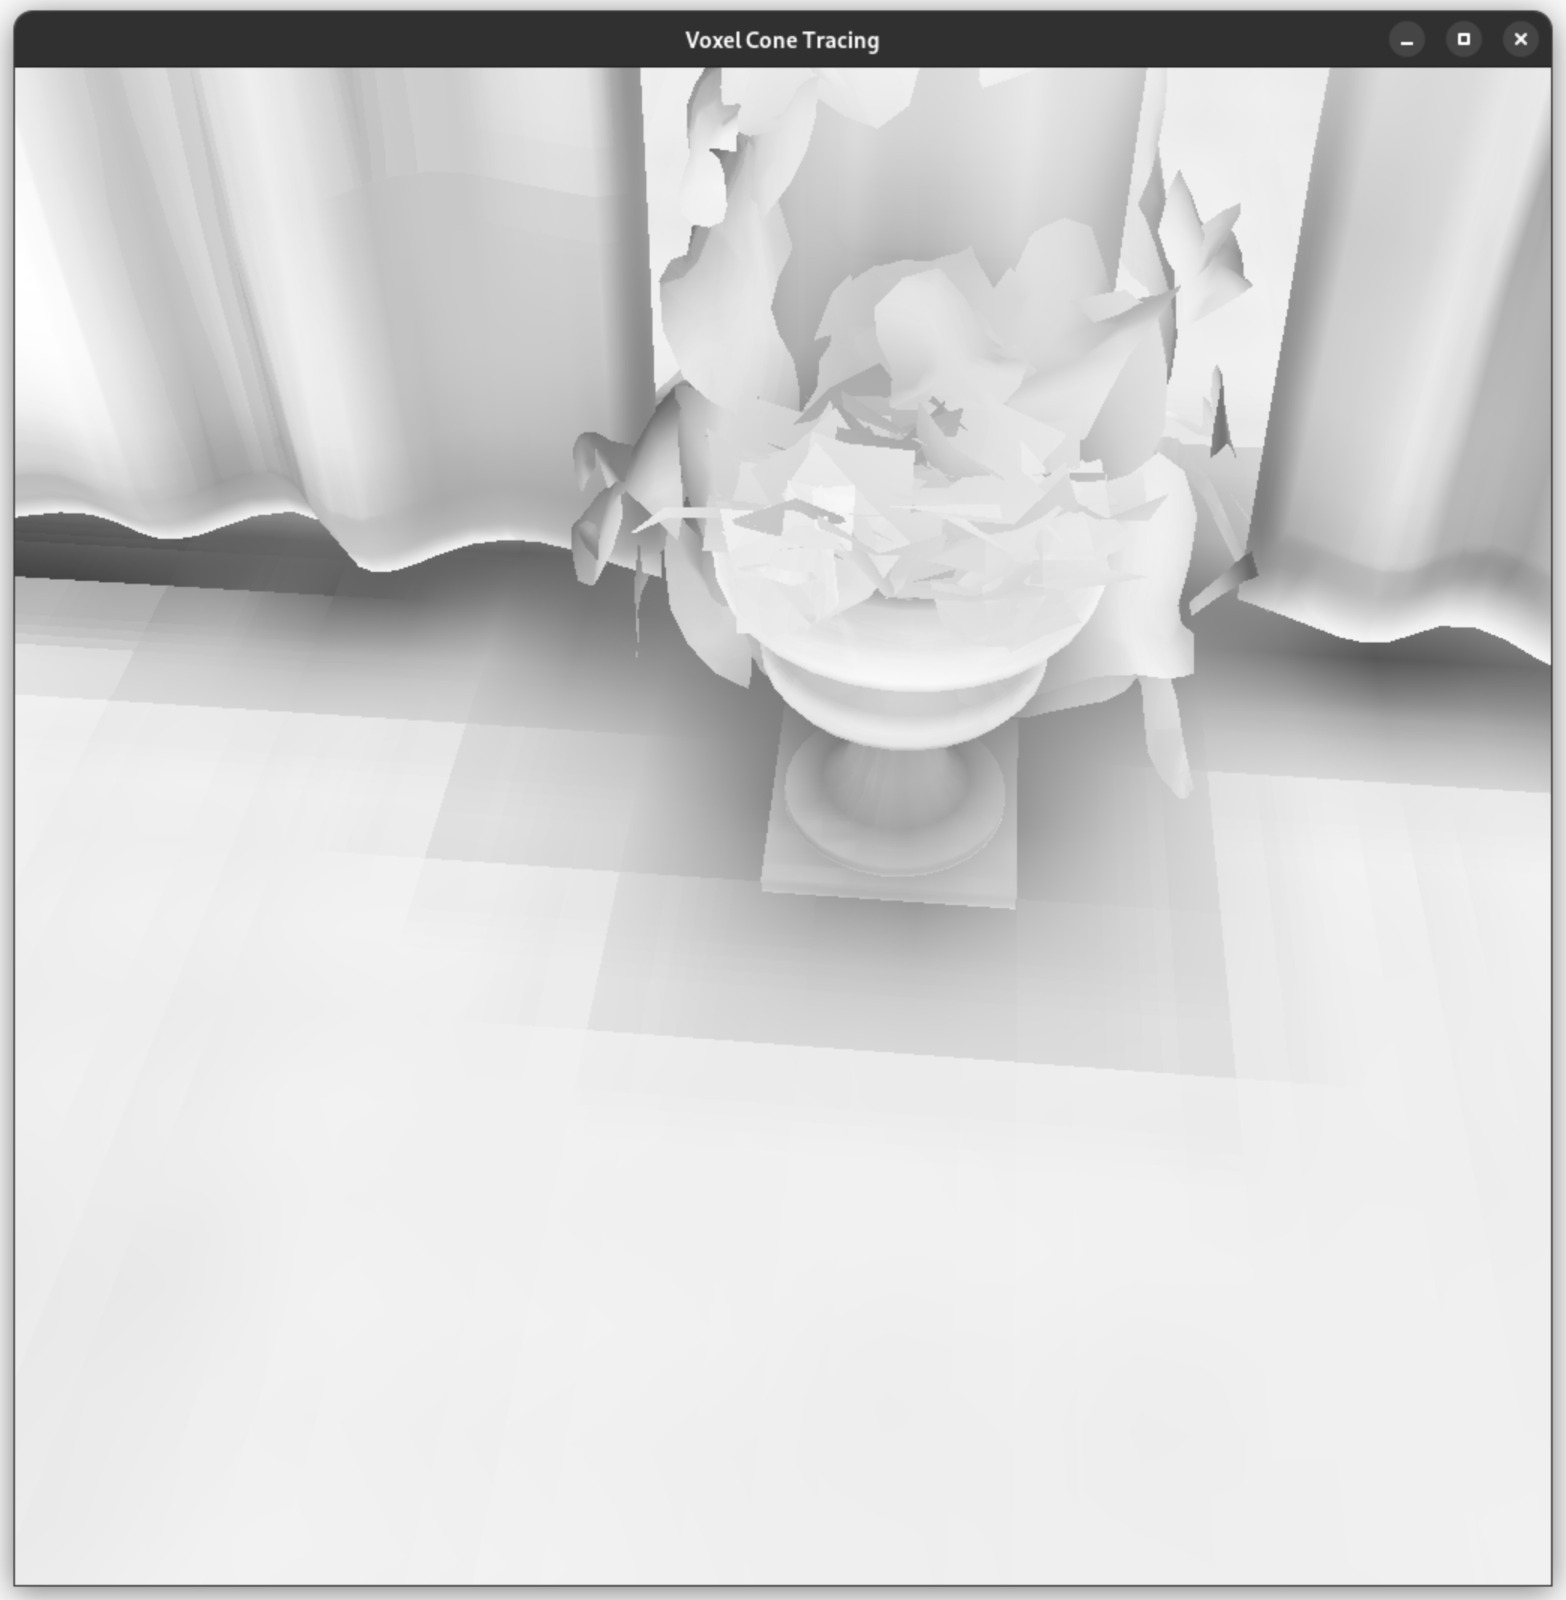
\includegraphics[width=.5\textwidth]{border-interpolation-issue.jpeg}
%     \caption{Falta de interpolación en la frontera entre geometría y espacio vacío}
%     \label{fig:border_interpolation_issue}
% \end{figure}

% La solución al problema de interpolación es agregar una capa de nodos ``frontera'' entre los nodos de la geometría y el espacio vacío.
% Estos nodos se crean sin ningún atributo, pero participan en el proceso de border transfer\ref{chap:design}, donde consiguen en su parte más cercana a su vecino, un poco de su color.
% Esto permite la interpolación correcta.

% TODO: Mostrar diagramita del border transfer resultante

% TODO: Agregar una foto de la misma situación pero arreglada.
% Tenemos que arreglar el AO para poder tener esto.

\subsection{Filtrado}\label{design:filtering}

Una vez que todos los atributos se encuentran en las hojas del octree, estos deben ser filtrados a posiciones superiores.
Filtrarlos implica promediarlos de tal manera que para un nodo no hoja $A$, lograr que su brick tenga un resumen de la información contenida en los bricks de todos sus hijos.
Esto se realiza en $n - 1$ pasos, con $n$ el máximo nivel del octree.
En cada paso, se calcula el valor de cada vóxel del brick del padre, usando los bricks de los hijos.

Consideremos un nodo de un nivel mayor al último, con su brick asociado y sus hijos, como muestra la figura \ref{fig:node_with_children}.
En este caso se muestran solo $4$ hijos porque es en 2D, en lugar de $8$ como en el caso tridimensional.
Cada hijo tiene a su vez su propio brick asociado como se muestra en la figura \ref{fig:all_child_bricks}.

\begin{figure}[h!]
    \centering
    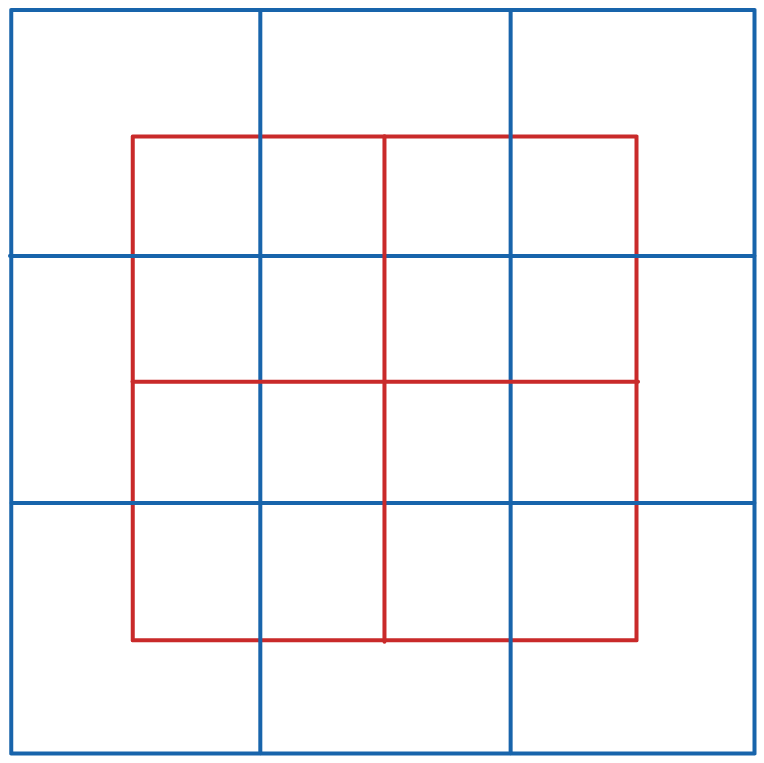
\includegraphics[width=.3\textwidth]{node-with-children.png}
    \caption{Nodo con su brick asociado y sus hijos}
    \label{fig:node_with_children}
\end{figure}

\begin{figure}[h!]
    \begin{center}
        \begin{subfigure}{.24\textwidth}
            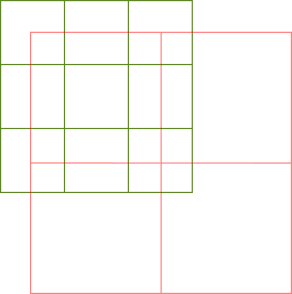
\includegraphics[width=\textwidth]{first-child-brick.png}
        \end{subfigure}
        \begin{subfigure}{.24\textwidth}
            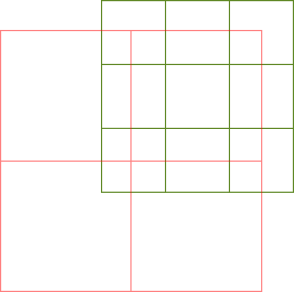
\includegraphics[width=\textwidth]{second-child-brick.png}
        \end{subfigure}
        \begin{subfigure}{.24\textwidth}
            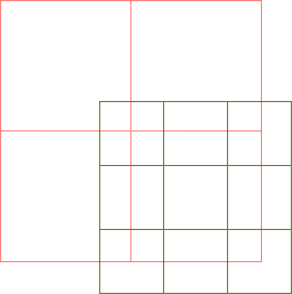
\includegraphics[width=\textwidth]{third-child-brick.png}
        \end{subfigure}
        \begin{subfigure}{.24\textwidth}
            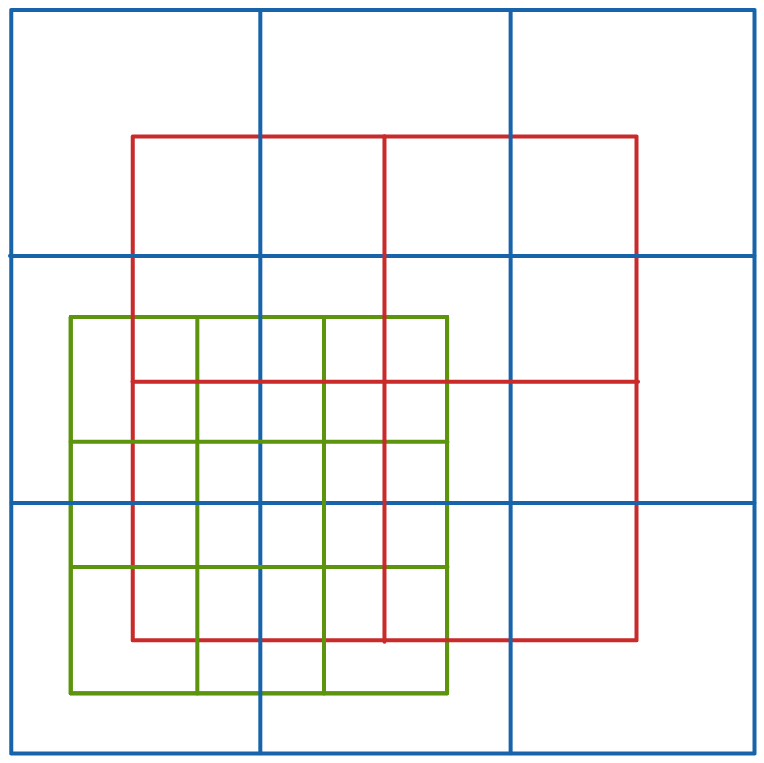
\includegraphics[width=\textwidth]{fourth-child-brick.png}
        \end{subfigure}
    \end{center}
    \caption{Bricks de todos los hijos del nodo}
    \label{fig:all_child_bricks}
\end{figure}

Los valores de los vóxeles se calculan en 4 pasajes distintos:
\begin{itemize}
    \item Esquinas
    \item Bordes
    \item Caras
    \item Centro
\end{itemize}

Cada uno de estos pasajes calcula un valor parcial de un tipo de vóxel.
Es parcial porque para los vóxeles limítrofes con otro nodo, este valor tiene que luego ser agregado con el de los vecinos.
Luego este valor parcial se utiliza \textit{border\_transfer} para conseguir los valores totales.

El cálculo para cada pasaje es el mismo para todos los vóxeles dentro de su grupo, así que se mostrará cómo se calcula solamente para un ejemplo tipo de cada grupo (esquinas, bordes, caras, centro.
En el caso 2D, no existe el vóxel centro.

Dado el vóxel superior izquierdo de la figura \ref{fig:svo_filtering_corners}, se considera solo el brick del hijo superior izquierdo del nodo.
De ese brick, se consideran los vóxeles iluminados.
El valor final del vóxel del padre se calcula promediando los valores de los vóxeles del hijo, pesados por el porcentaje de solapamiento.
Esto resulta en un kernel gaussiano. % TODO: Alguna referencia sobre kernels gaussianos? Si no no lo mencionamos

\begin{figure}
    \centering
    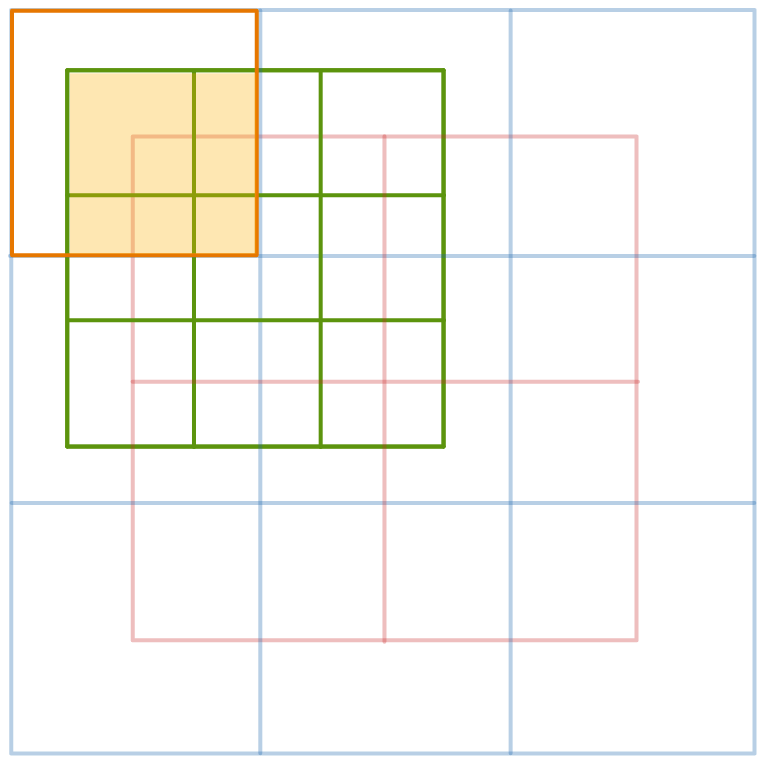
\includegraphics[width=.5\textwidth]{svo-filtering-corner.png}
    \caption{Filtrado para un vóxel esquina}
    \label{fig:svo_filtering_corners}
\end{figure}

De la misma manera se calculan los vóxels de los bordes y de las caras, solo que en esos casos se usan más de un brick hijo, como se puede ver en las figuras \ref{fig:svo_filtering_edges} y \ref{fig:svo_filtering_faces}.

\begin{figure}
    \begin{center}
        \begin{subfigure}{.49\textwidth}
            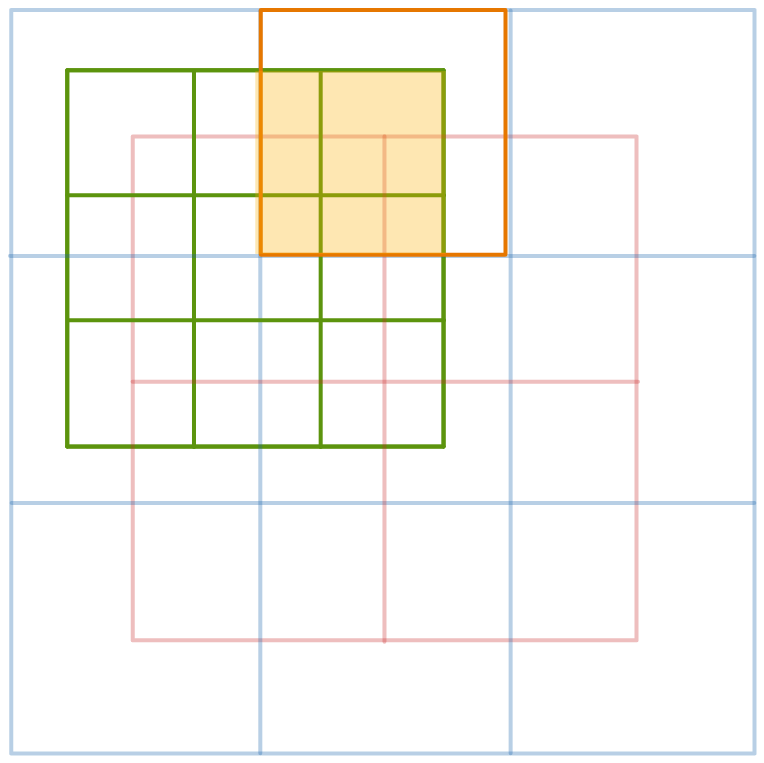
\includegraphics[width=\textwidth]{svo-filtering-edge-1.png}
        \end{subfigure}
        \begin{subfigure}{.49\textwidth}
            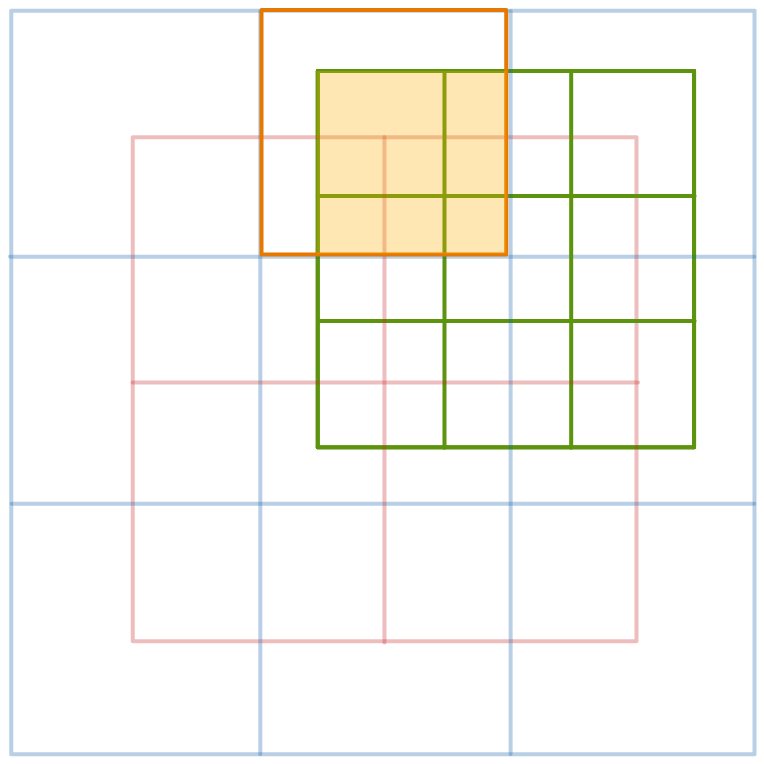
\includegraphics[width=\textwidth]{svo-filtering-edge-2.png}
        \end{subfigure}
    \end{center}
    \caption{Filtrado para un vóxel borde}
    \label{fig:svo_filtering_edges}
\end{figure}

\begin{figure}
    \begin{center}
        \begin{subfigure}{.24\textwidth}
            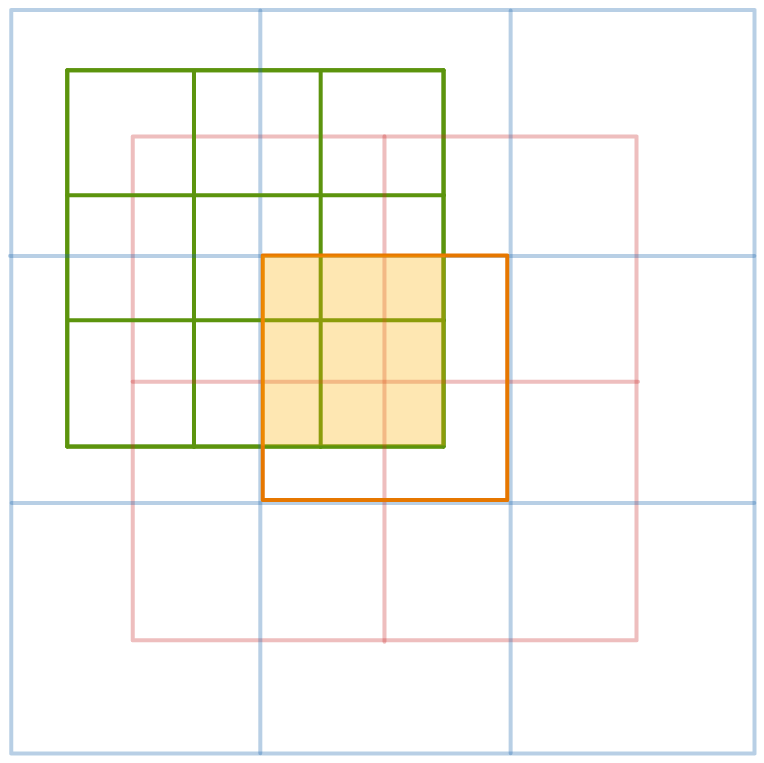
\includegraphics[width=\textwidth]{svo-filtering-face-1.png}
        \end{subfigure}
        \begin{subfigure}{.24\textwidth}
            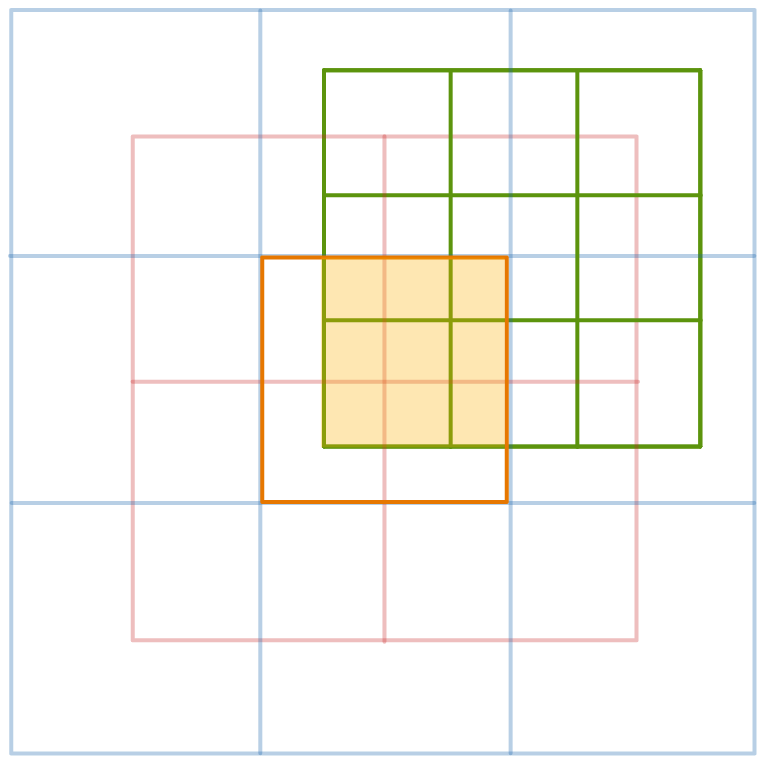
\includegraphics[width=\textwidth]{svo-filtering-face-2.png}
        \end{subfigure}
        \begin{subfigure}{.24\textwidth}
            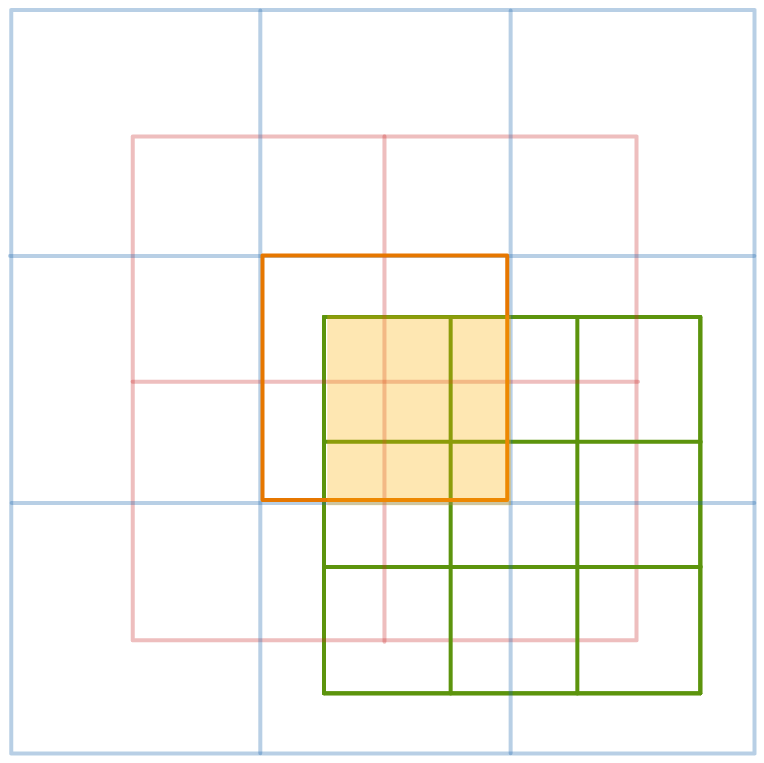
\includegraphics[width=\textwidth]{svo-filtering-face-3.png}
        \end{subfigure}
        \begin{subfigure}{.24\textwidth}
            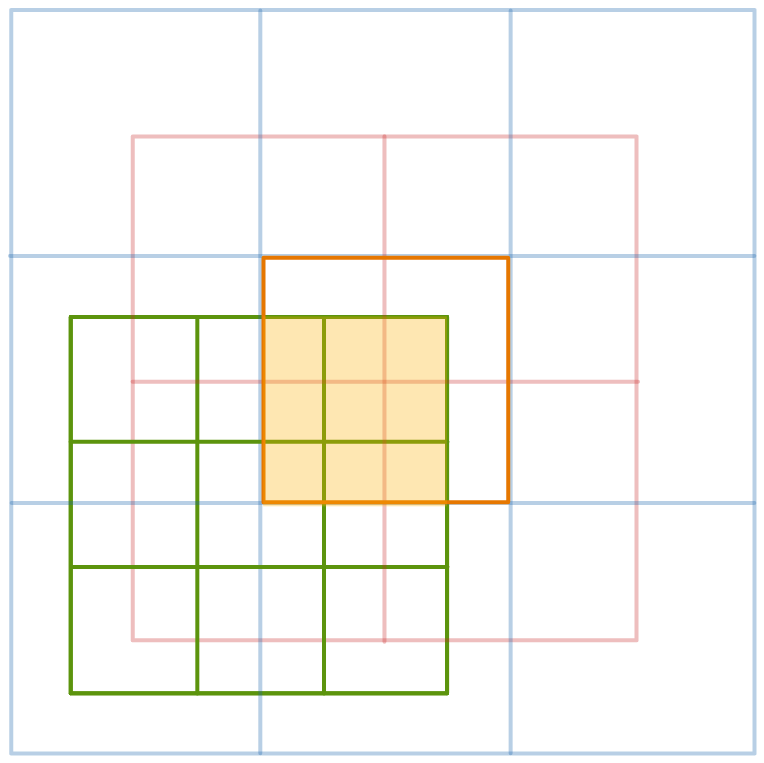
\includegraphics[width=\textwidth]{svo-filtering-face-4.png}
        \end{subfigure}
    \end{center}
    \caption{Filtrado para un vóxel cara}
    \label{fig:svo_filtering_faces}
\end{figure}

% TODO: Solo traer de vuelta si realmente usamos normales en el código.
% Si los vóxels almacenan normales, estas se promedian como se mencionó en la sección \ref{sec:normal_filtering}.

\subsection{Filtrado anisotrópico}

El filtrado descrito en la sección anterior resulta en vóxeles cuyos valores son los mismos vistos en todas las direcciones.
A pesar de que el vóxel es un cubo, almacena solo un valor, en lugar de tener distintos valores según de dónde se mira.
Esto es muy útil a la hora de representar un atributo como el color en una escena 3D.

Consideremos un vóxel de un nodo alto en el árbol, que representa una gran región del espacio.
Esta región contiene únicamente una pared que pasa por su centro, y el resto es todo espacio vacío.
En este caso, entonces visto de la dirección paralela a la normal de la pared, el vóxel se verá del color de la pared y será completamente opaco, mientras que visto de la dirección perpendicular a la normal de la pared, el vóxel será completamente transparente.
Esta situación se muestra en la figura \ref{fig:anisotropic-thin-wall}.

Este comportamiento no ocurre con el filtrado anterior, que se conoce como isotrópico, significando ``igual en todas las direcciones del espacio''.
La solución es mejorar el filtrado y hacerlo 6 veces por vóxel, uno por cada dirección alineada con los ejes, X, -X, Y, -Y, Z, -Z.
Luego, se puede usar la dirección de vista para interpolar usando las tres direcciones más cercanas.
Este comportamiento es anisotrópico, no es igual para todas las direcciones.

\begin{figure}
    \begin{center}
        \begin{subfigure}{.24\textwidth}
            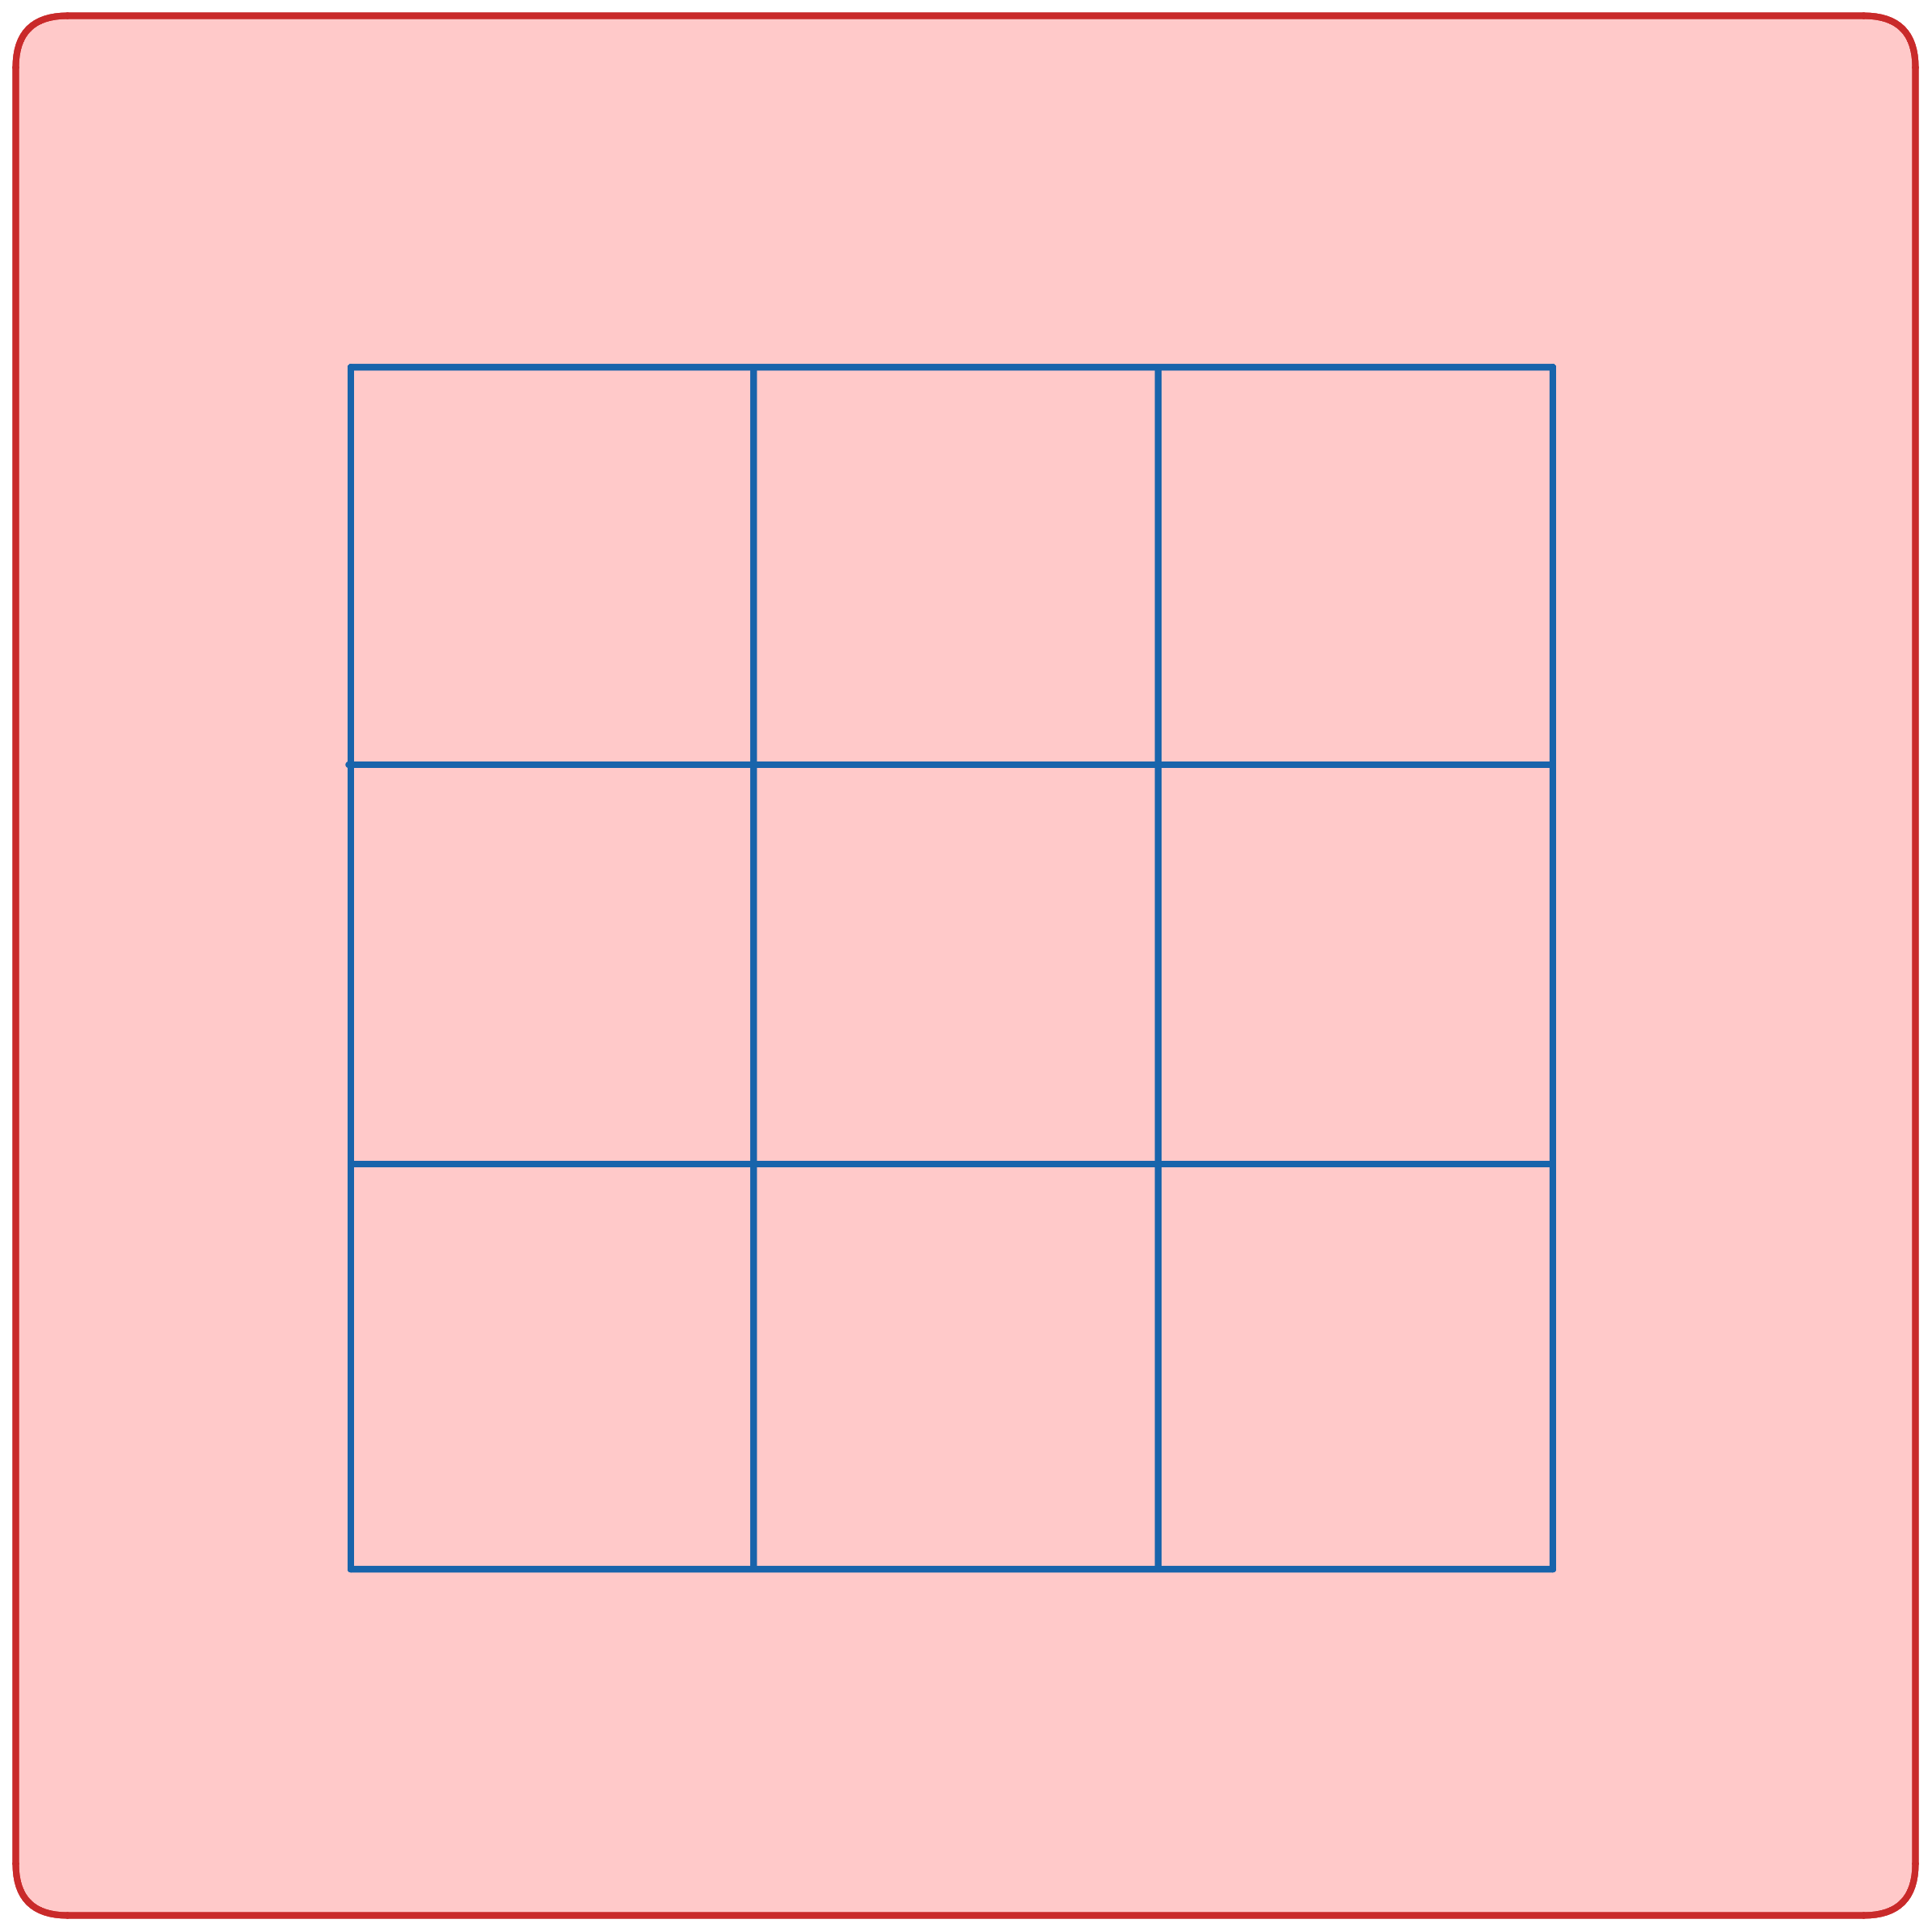
\includegraphics[width=\textwidth]{anisotropic-filtering-thin-wall-front.png}
            \caption{Visto de frente}
        \end{subfigure}
        \begin{subfigure}{.24\textwidth}
            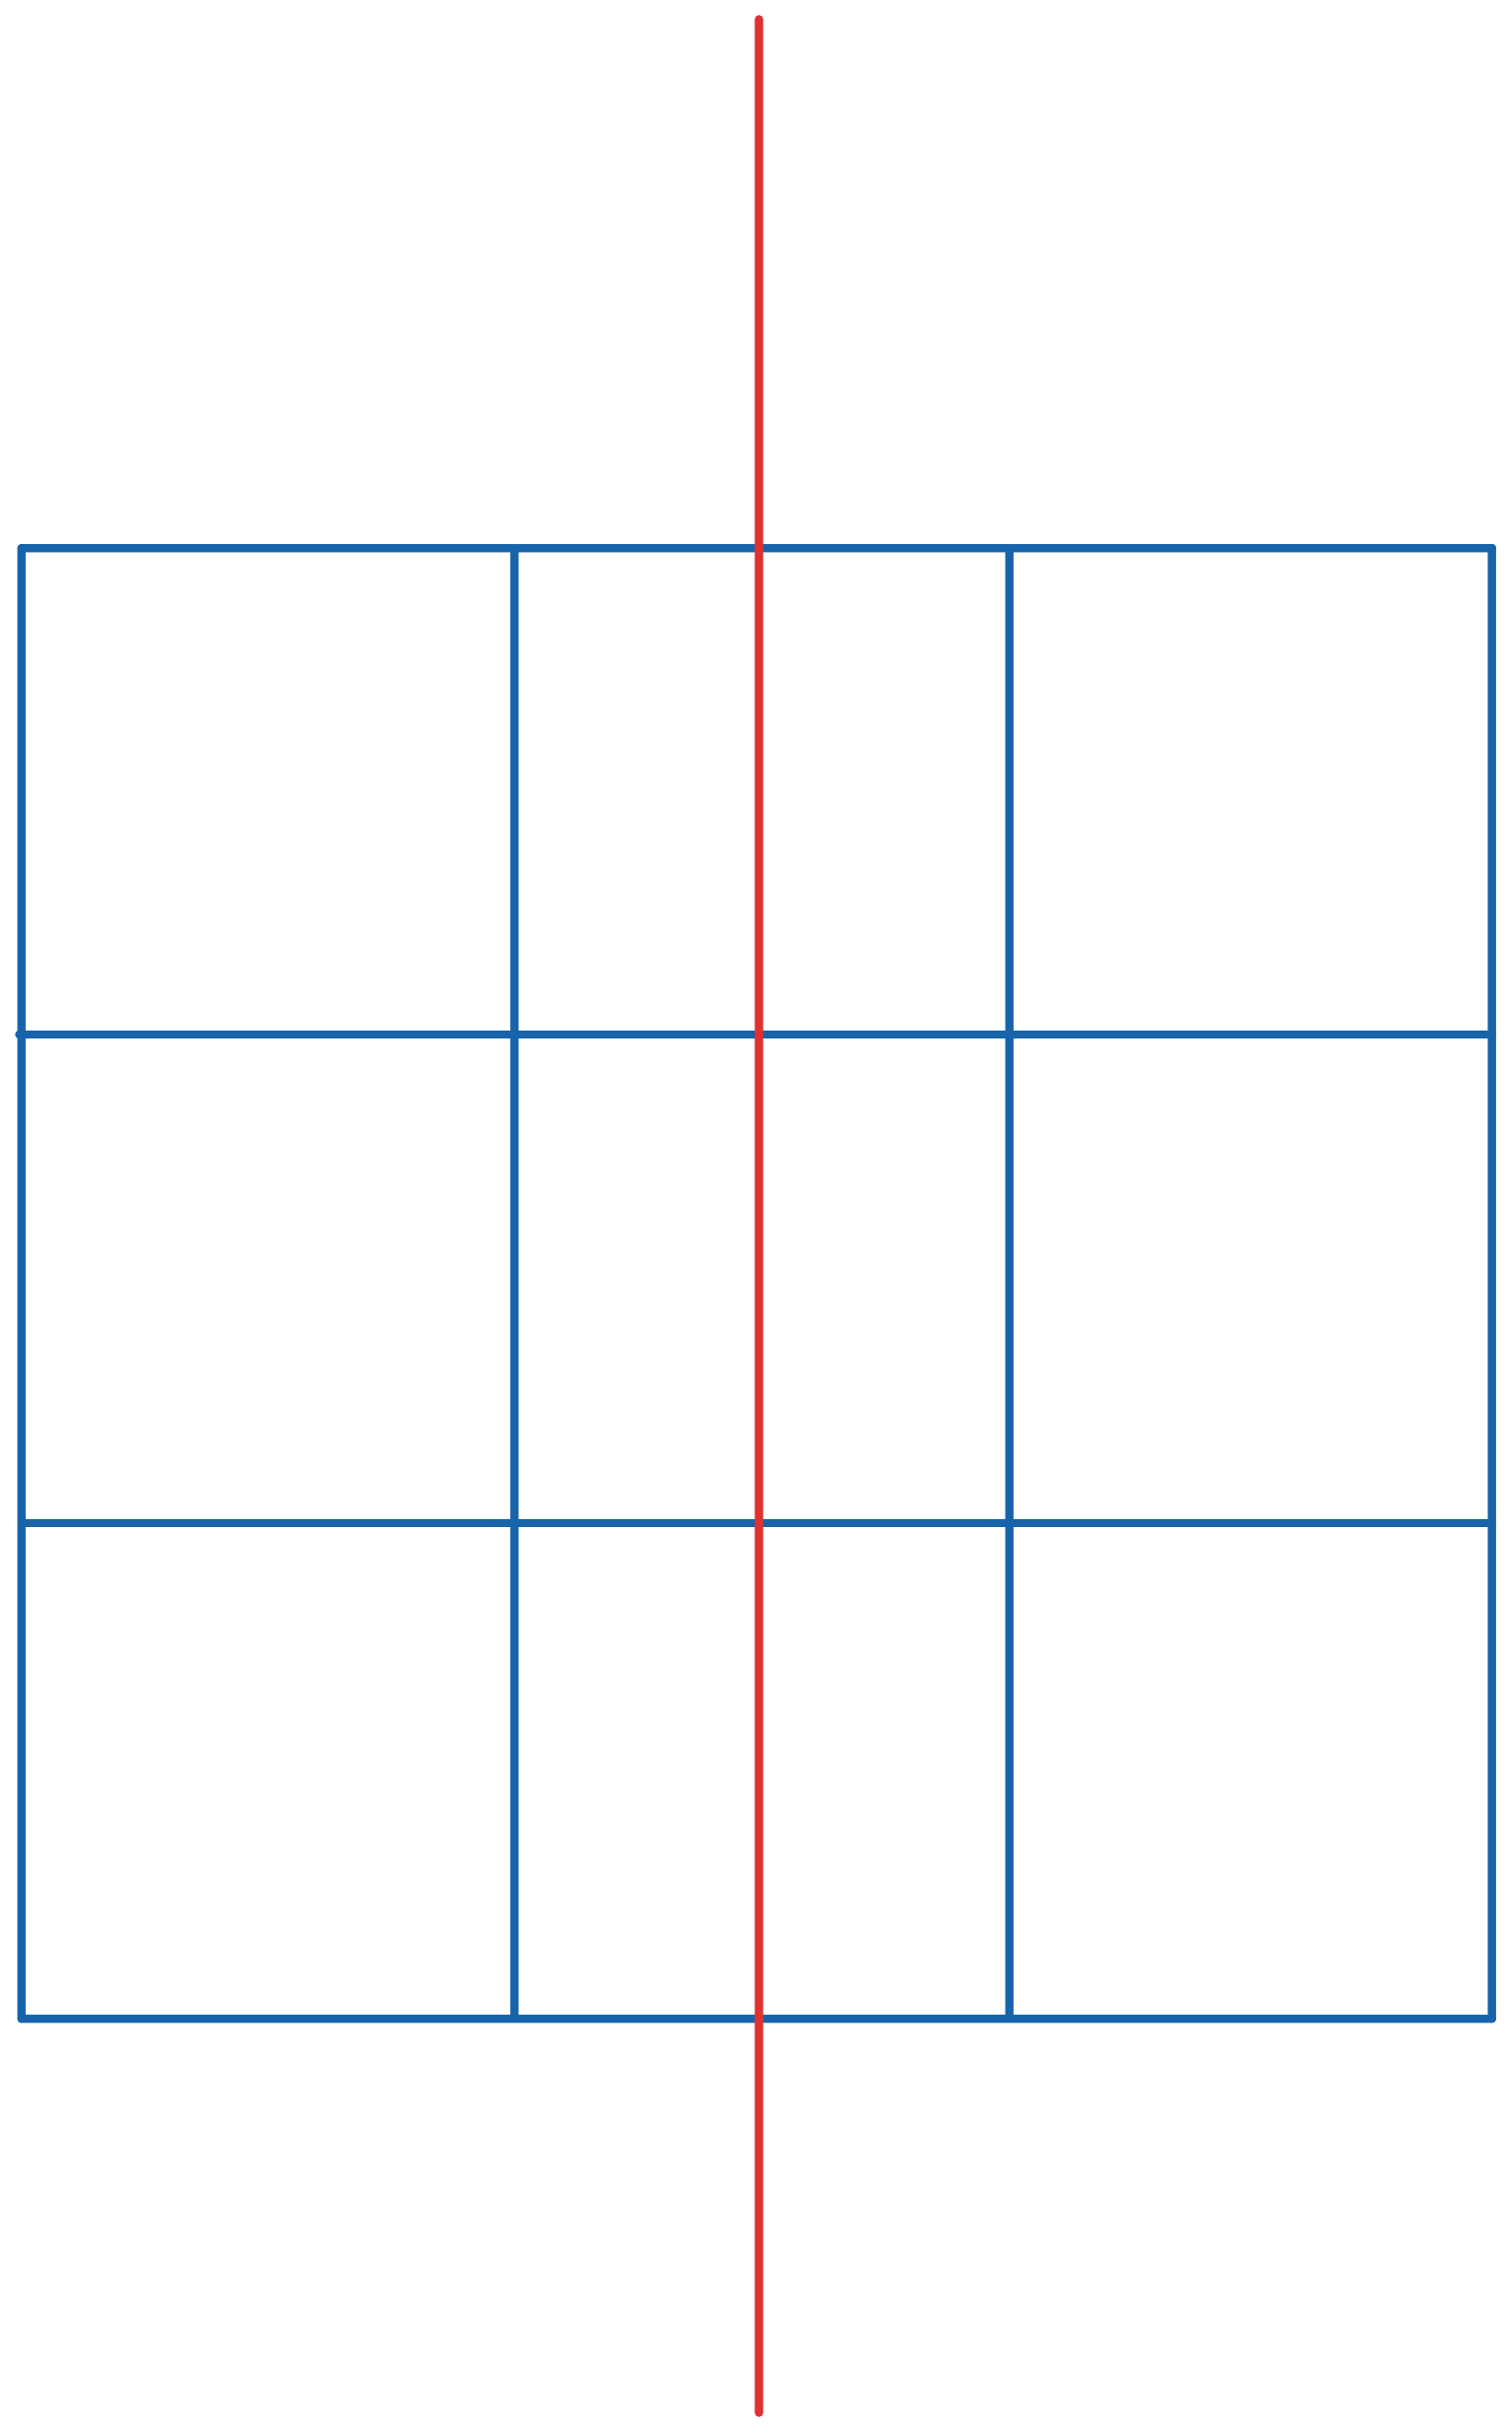
\includegraphics[width=\textwidth]{anisotropic-filtering-thin-wall-side.png}
            \caption{Visto de costado}
        \end{subfigure}
        \caption{Brick que contiene una pared fina}
        \label{fig:anisotropic-thin-wall}
    \end{center}
\end{figure}

Dada una dirección, por ejemplo, de izquierda a derecha, se encuentra una base de vóxeles y se usan para calcular \textbf{valores direccionales}.
En la figura \ref{fig:svo_filtering_anisotropic} se pueden ver todos los valores direccionales que deben ser calculados para un brick en 2D, para todas las direcciones.
Para cada vóxel de la base, se ejecuta un algoritmo de acumulación de opacidad que va avanzando en la dirección dada.
Si el algoritmo llega a opacidad 1, termina y devuelve el valor direccional para ese vóxel base.
Este algoritmo es el que soluciona situaciones como la de la pared mencionada anteriormente.

\begin{figure}
    \begin{center}
        \begin{subfigure}{.24\textwidth}
            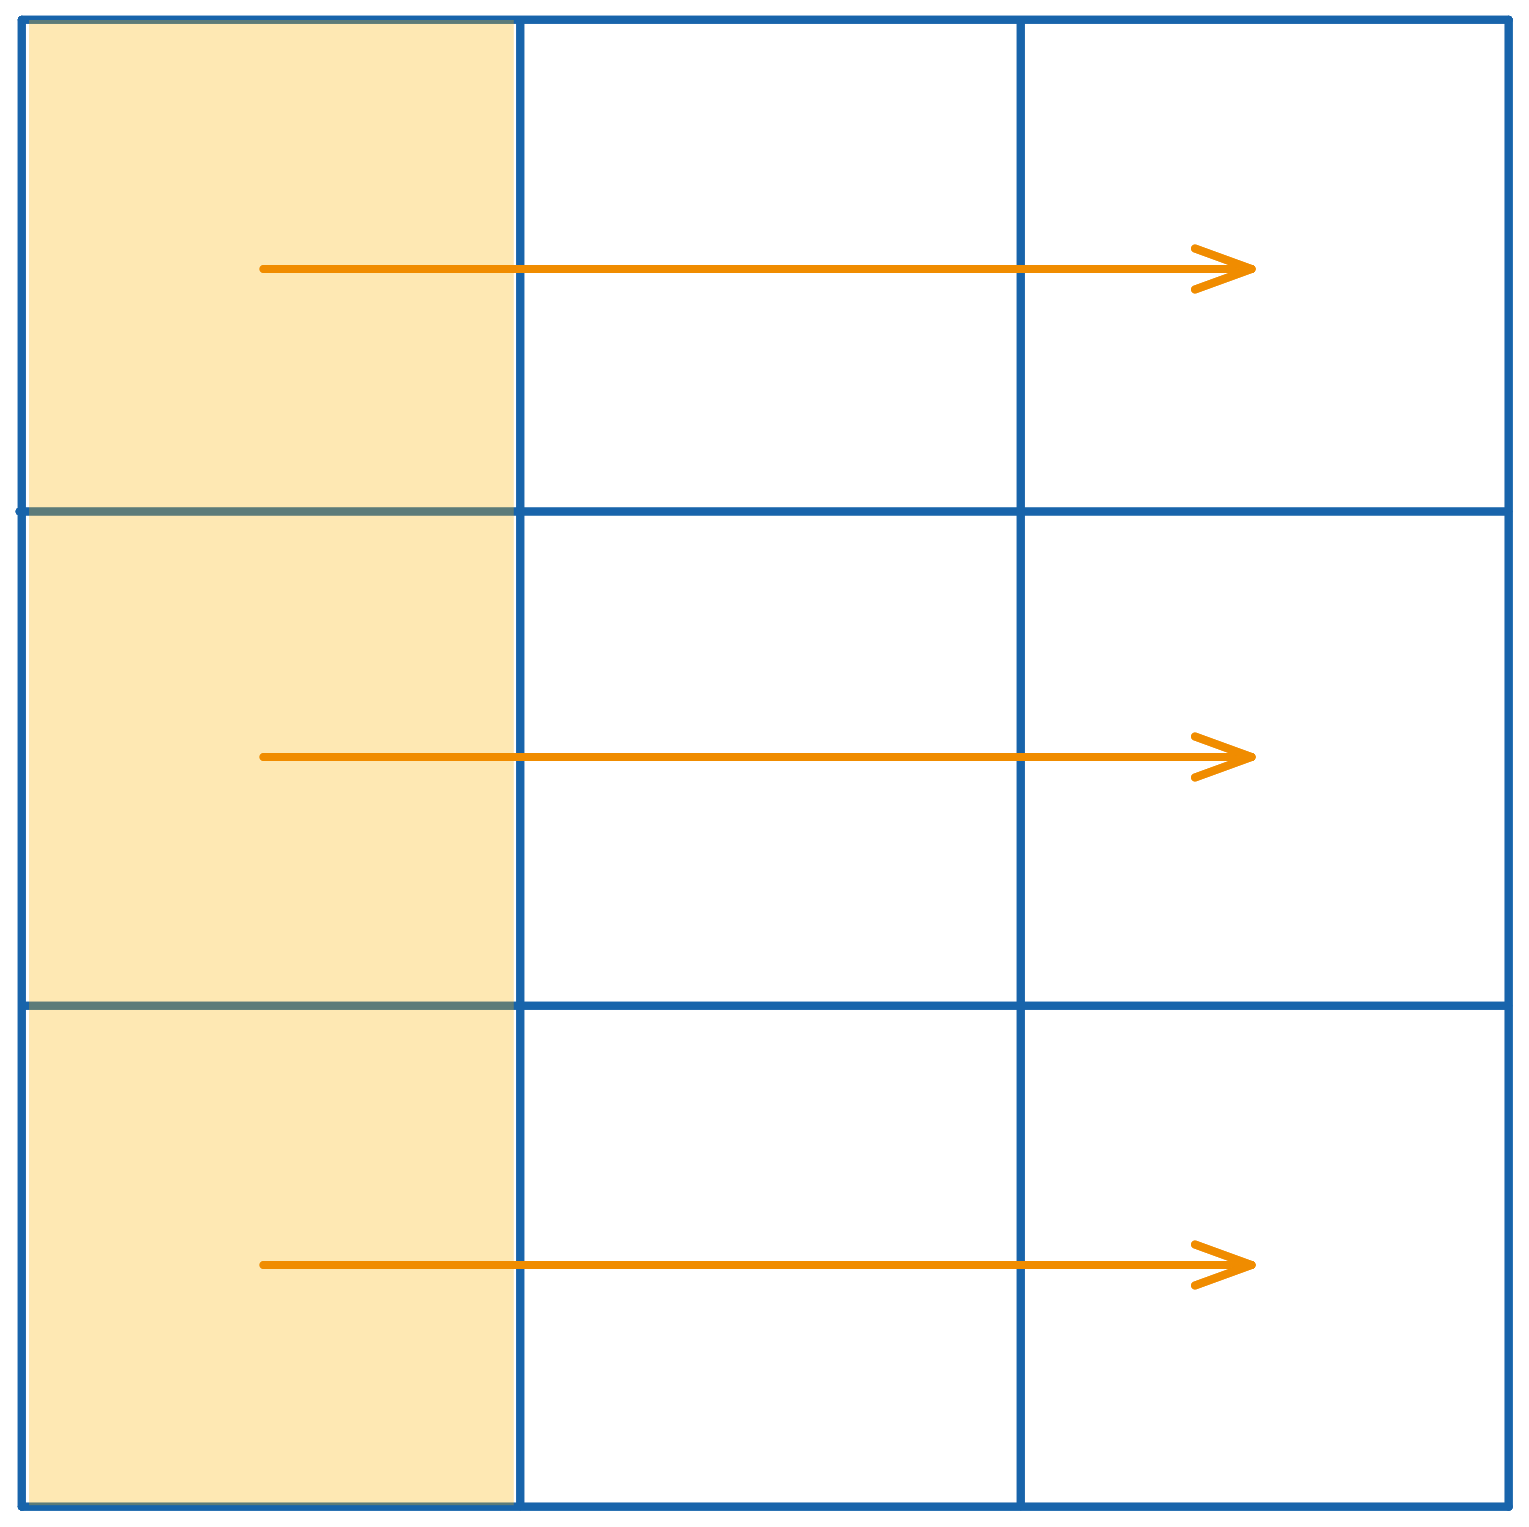
\includegraphics[width=\textwidth]{anisotropic-filtering-x.png}
        \end{subfigure}
        \begin{subfigure}{.24\textwidth}
            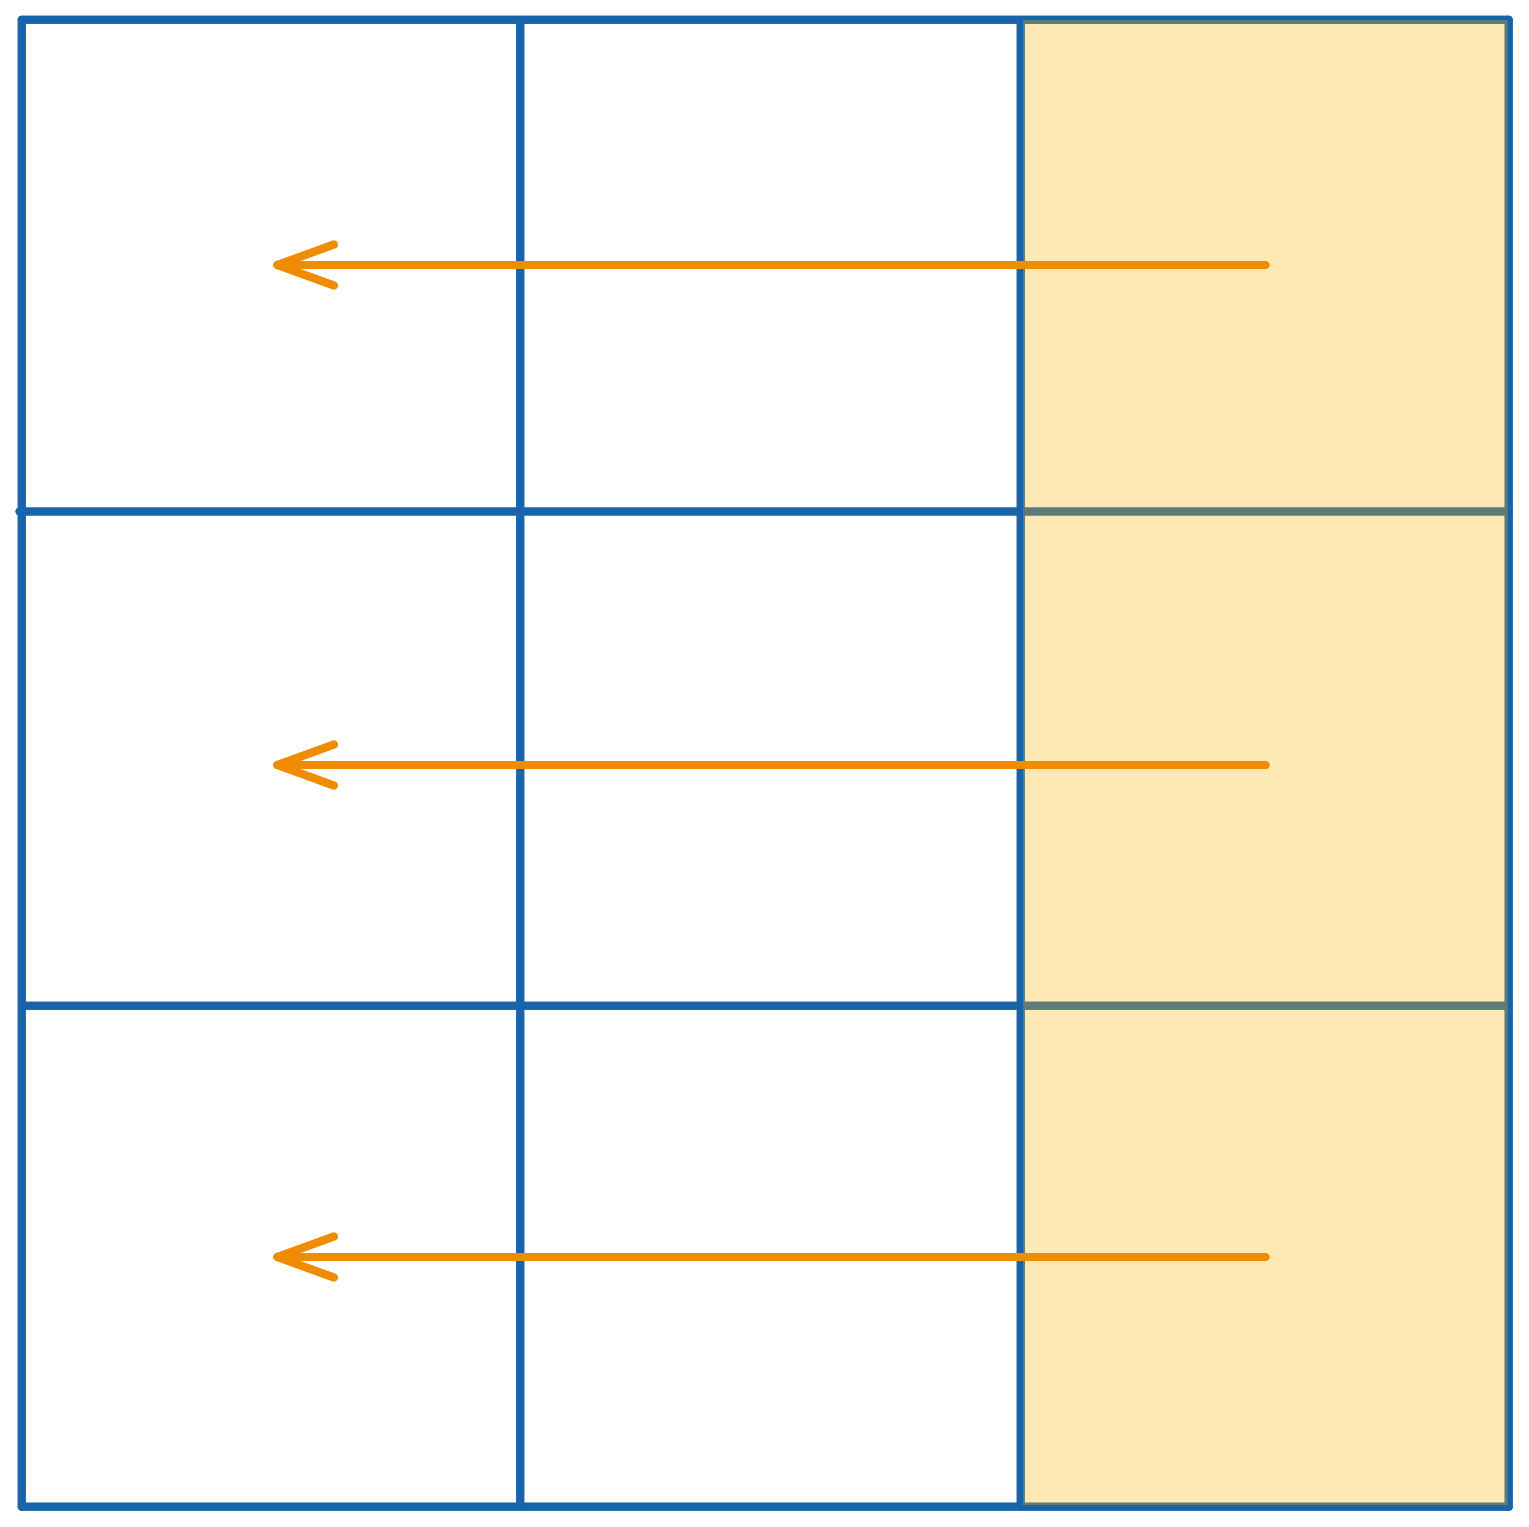
\includegraphics[width=\textwidth]{anisotropic-filtering-x-neg.png}
        \end{subfigure}
        \begin{subfigure}{.24\textwidth}
            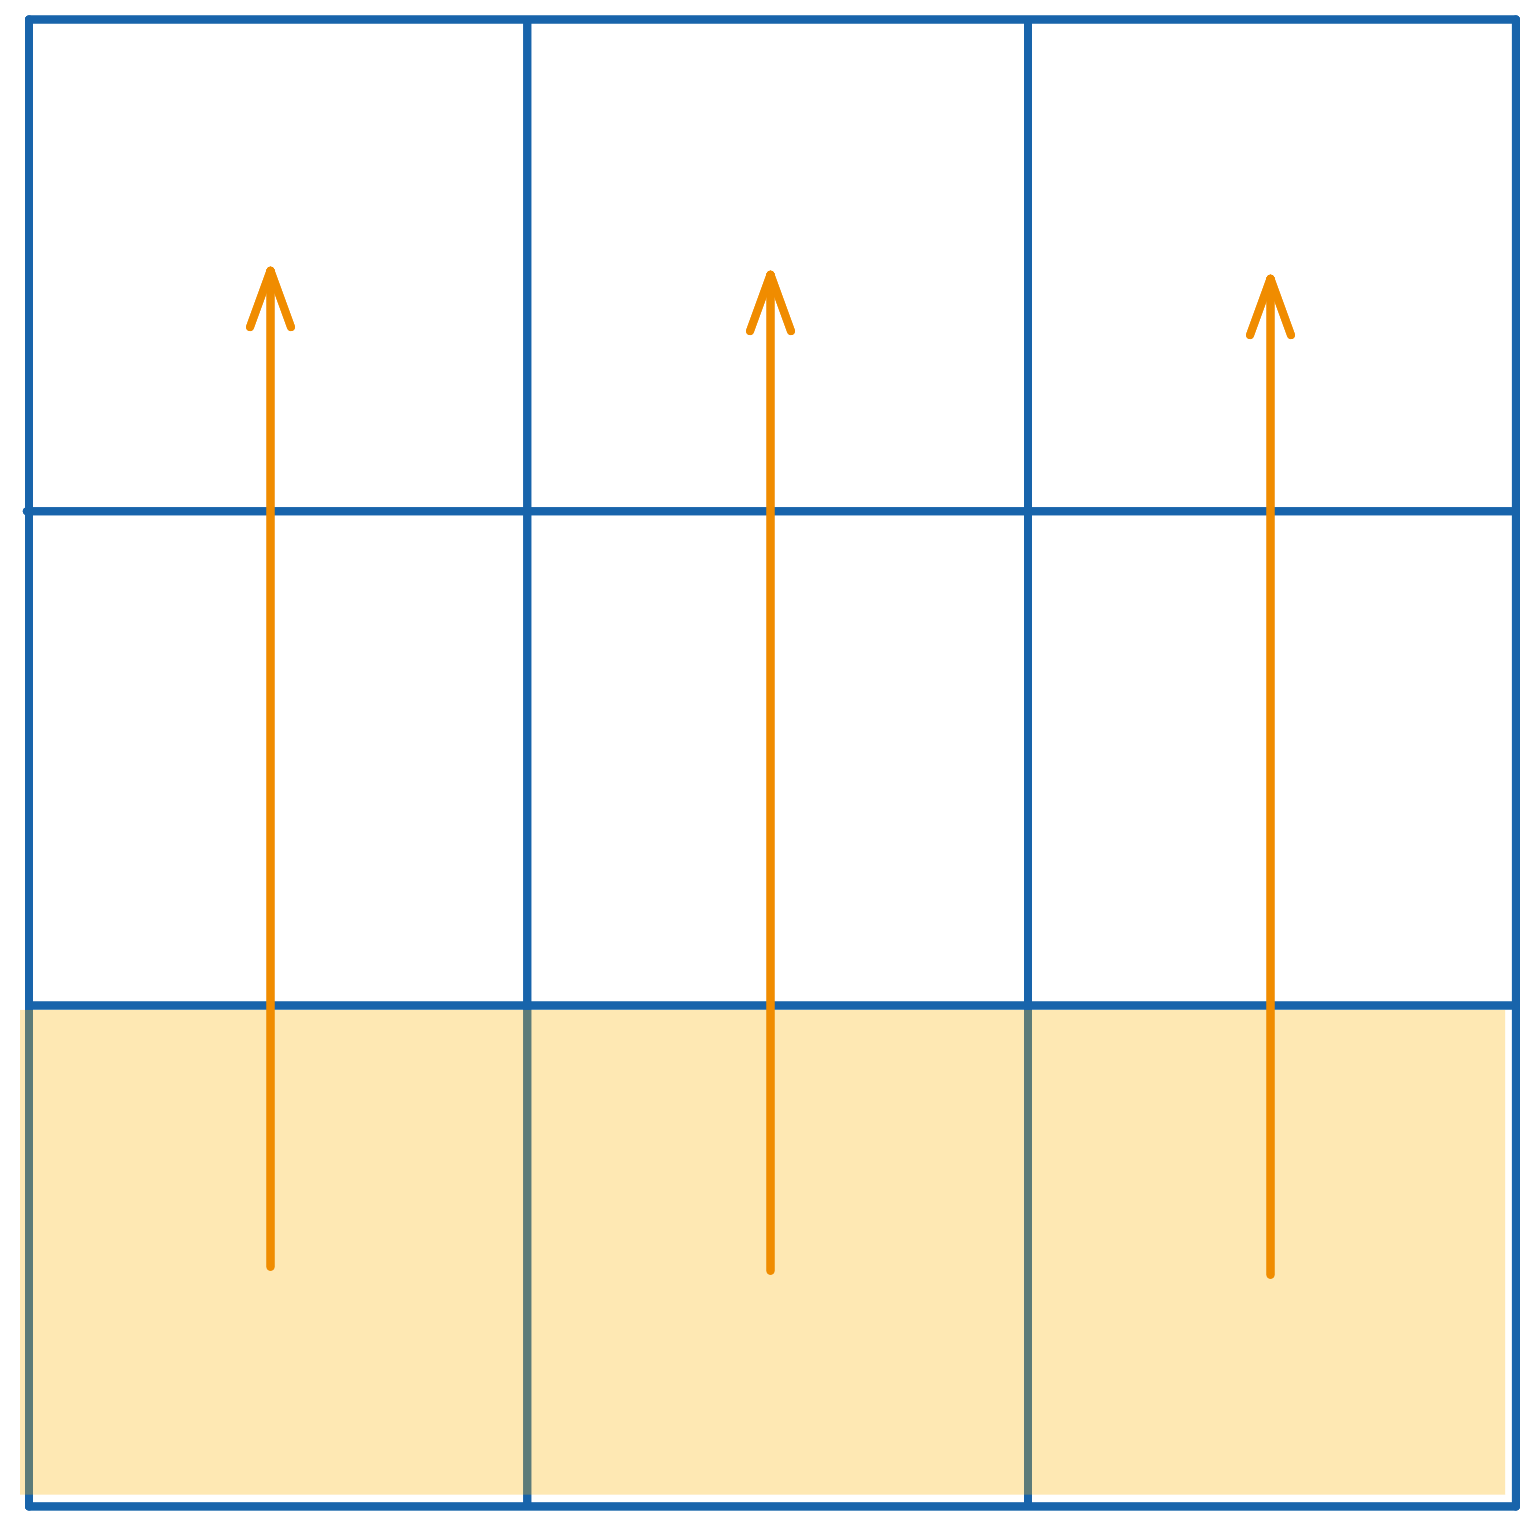
\includegraphics[width=\textwidth]{anisotropic-filtering-y.png}
        \end{subfigure}
        \begin{subfigure}{.24\textwidth}
            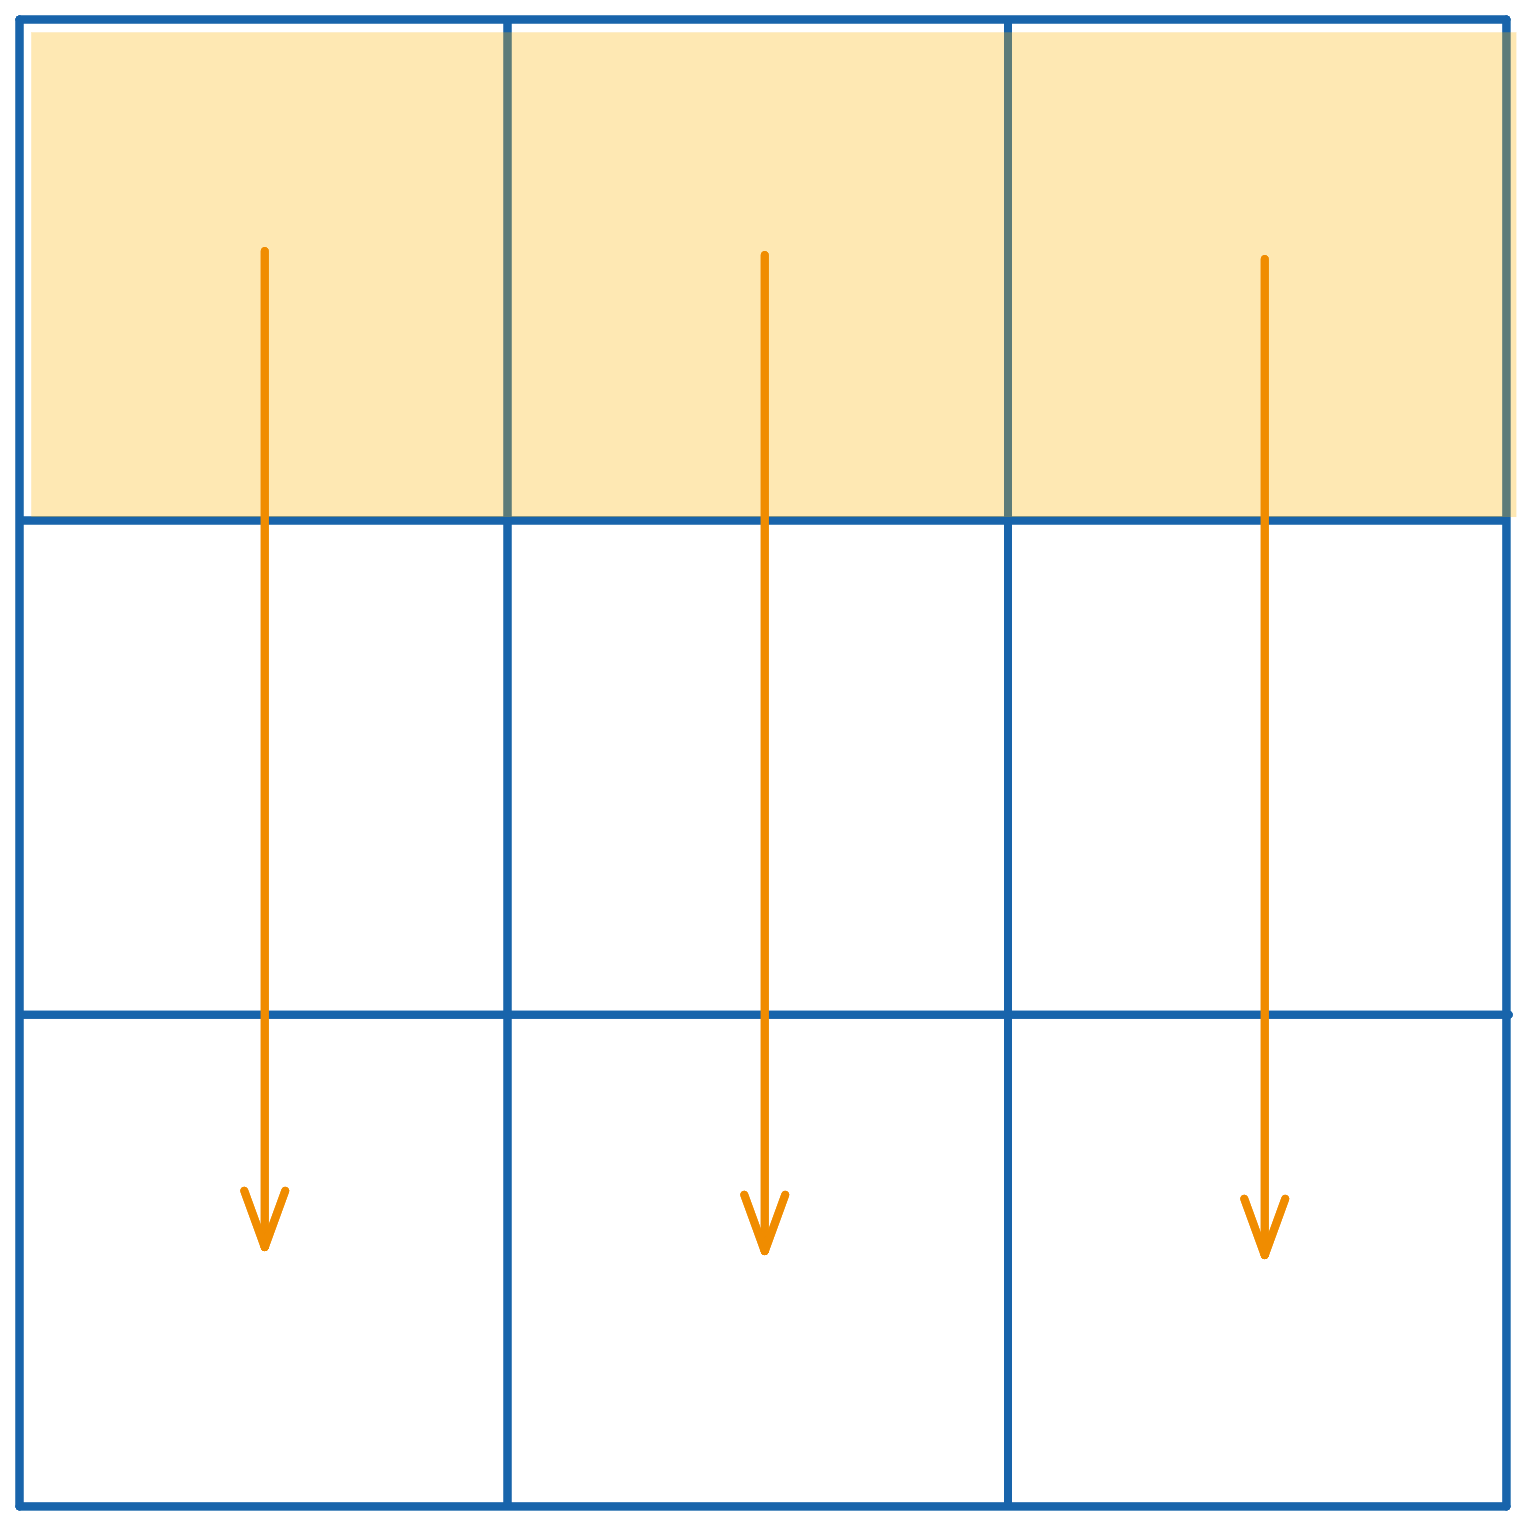
\includegraphics[width=\textwidth]{anisotropic-filtering-y-neg.png}
        \end{subfigure}
    \end{center}
    \caption{Filtrado anisotrópico en todas las direcciones}
    \label{fig:svo_filtering_anisotropic}
\end{figure}

\section{Cone tracing}\label{sec:cone_tracing}

% Antes de comenzar con el algoritmo de cone tracing, es de utilidad implementar deferred shading \cite{deferred-shading}.
% Esta técnica utiliza el pipeline de renderizado para generar múltiples texturas con los atributos deseados desde el punto de vista de la cámara.
% Luego, son estas texturas la que se usan como entrada al algoritmo, en lugar de todos los vértices de la geometría de la escena.
% Estas texturas se conocen como \textit{geometry buffers}.
% Al ya usar el pipeline gráfico para escribir los atributos en una textura intermedia, ya se descartan fragmentos no visibles desde la cámara.
% Esto reduce la cantidad de cálculos necesarios.

La entrada al algoritmo de cone tracing no son los vértices de la escena, si no los \textit{geometry buffers} que contienen los valores de la escena ya habiendo descartado los vértices fuera de vista, como se explicó en \ref{sec:forward_vs_deferred}.

El algoritmo de cone tracing es ejecutado para cada píxel de los geometry buffers para calcular un color que se escribe en otra textura, la que finalmente se muestra sobre un quad que cubre toda la pantalla.

Dado un punto de origen, se lanza uno o varios conos con cierta dirección y apertura, dependiendo del efecto que se quiere lograr.
% TODO: Tema de las normales
% todo considerando el hemisferio hacia el lado de la normal del punto.

Dado un cono, se parte desde su origen y se avanza en su dirección con un cierto tamaño de paso.
% TODO: Acá estaría bueno poder linkear a algo de ray marching
Después de cada paso tomado, se calcula el diámetro del cono en ese punto.
Dado el diámetro, se calcula un nivel del octree, y dado ese nivel y la posición a lo largo del cono, se recorre el octree y se encuentra el nodo que corresponde a ese nivel y a esa posición.
Ese nodo tiene un brick asociado, cuyos vóxeles tienen los valores prefiltrados, conseguidos en \ref{design:filtering}.
Se usa el valor del vóxel que corresponde con la posición y se acumula.
Se sigue avanzando paso a paso en el cono acumulando valores hasta satisfacer un criterio de parada.
El algoritmo de cone tracing en si es simple dado todos los pasos anteriores.

\section{Efectos}

Dependiendo de la cantidad, el tamaño, la dirección y el criterio de parada de los conos, se pueden lograr varios efectos con cone tracing.

\subsection{Oclusión ambiental}

La oclusión ambiental es una técnica de rendering que se usa para calcular qué tan expuesto está cada punto de una escena a la luz ambiental.
Cone tracing se puede usar para calcular este valor.
Este efecto no aporta más al realismo de una escena una vez que se usan los de iluminación indirecta, pero es un buen paso previo para ver el funcionamiento del algoritmo.

Para calcularlo, se lanzan varios conos, cubriendo el hemisferio centrado en la normal del punto.
El único valor necesario es la opacidad.
A medida que se va viajando a lo largo de un cono, se va acumulando la opacidad de los vóxels que se tocan.
Se define una distancia máxima y el criterio de parada es cuando el punto a lo largo del cono pasa esa distancia máxima.

\subsection{Conos de sombra}

De la misma manera que el trazado de rayos logra sombras lanzando un rayo hacia la fuente de luz, en este caso se logran lanzando un cono hacia la fuente de luz.
El cono toma en cuenta únicamente la opacidad y su criterio de parada es alcanzar la luz o 1 de opacidad antes.
El beneficio de que sea un cono en lugar de un rayo es que se logran sombras suaves, sin necesidad de tener que tomar muchas muestras y promediarlas.

\subsection{Iluminación indirecta}

Para producir efectos de iluminación indirecta, se toma un enfoque parecido al de \textit{photon mapping}, y se lanzan fotones a partir de la fuente de luz.

Para hacer esto, se renderiza la escena desde cada fuente de luz, con esto se genera un mapa de luz.
Todos los mapas de luz se guardan en texturas, donde se almacena, para cada texel de la textura, la posición global de la geometría.
Luego, cada una de estas texturas se recorren texel a texel y se recorre el octree para guardar en el brick correspondiente un fotón.
Con esto, se almacenan en todas las hojas del octree fotones.
Estos fotones se transfieren a través de las fronteras (esta vez sumando y no promediando) y se filtran al igual que los otros atributos.

Con esta información de iluminación, se pueden generar reflejos.

\subsubsection{Reflejos difusos}

Para reflejos difusos, se lanzan conos para cubrir el hemisferio centrado en la normal del punto.
En la mayoría de los casos, 5 conos anchos difusos dan un buen resultado.
Cada cono acumula el color de los vóxeles con los que se encuentra multiplicado por la cantidad de fotones.
Esto logra un efecto de \textit{light bleed}, donde las superficies adquieren color de otras superficies cercanas que reciben luz.

\subsubsection{Reflejos especulares}

Para los reflejos especulares, se lanza un solo cono fino en la dirección de reflexión.
Este cono, al ser más fino, se encuentra con nodos de niveles más bajos, con lo que el reflejo tiene mejor definición.

% END.

% La parte central del trabajo refiere a lo que es producción propia o aporte del
% proyecto de grado, incluyendo las decisiones tomadas. Por ejemplo, puede incluir
% los requerimientos, el análisis y el diseño de la solución. Si el proyecto tiene una
% implementación, debe describirse en términos de decisiones tomadas en ese sentido.
% Los detalles de programación se dejan para los anexos.

% Se pueden incluir figuras en el documento, las mismas deben estar referenciadas en el texto. Por ejemplo, la Figura~\ref{fig:logos} muestra los logos de Facultad de Ingeniería y de la Universidad de la República.

% \begin{figure}[h!]
%     \centering
%     
\includegraphics[width=\textwidth]{figs/logo-udelar-fing.png}
%     \caption{Logos de FIng y UdelaR}
%     \label{fig:logos}
% \end{figure}
